%%%%%%%%%%%%%%%%%%%%%%%%%%%%%%%%%%%%%%%%%
% Masters/Doctoral Thesis 
% LaTeX Template
% Version 1.43 (17/5/14)
%
% This template has been downloaded from:
% http://www.LaTeXTemplates.com
%
% Original authors:
% Steven Gunn 
% http://users.ecs.soton.ac.uk/srg/softwaretools/document/templates/
% and
% Sunil Patel
% http://www.sunilpatel.co.uk/thesis-template/
%
% License:
% CC BY-NC-SA 3.0 (http://creativecommons.org/licenses/by-nc-sa/3.0/)
%
% Note:
% Make sure to edit document variables in the Thesis.cls file
%
%%%%%%%%%%%%%%%%%%%%%%%%%%%%%%%%%%%%%%%%%

%----------------------------------------------------------------------------------------
%	PACKAGES AND OTHER DOCUMENT CONFIGURATIONS
%----------------------------------------------------------------------------------------

\documentclass[11pt, oneside]{Thesis} % The default font size and one-sided printing (no margin offsets)

\graphicspath{{Pictures/}} % Specifies the directory where pictures are stored

\usepackage[square, numbers, comma, sort&compress]{natbib} % Use the natbib reference package - read up on this to edit the reference style; if you want text (e.g. Smith et al., 2012) for the in-text references (instead of numbers), remove 'numbers' 
\hypersetup{urlcolor=blue, colorlinks=true} % Colors hyperlinks in blue - change to black if annoying
\title{\ttitle} % Defines the thesis title - don't touch this

\begin{document}

\frontmatter % Use roman page numbering style (i, ii, iii, iv...) for the pre-content pages

\setstretch{1.3} % Line spacing of 1.3

% Define the page headers using the FancyHdr package and set up for one-sided printing
\fancyhead{} % Clears all page headers and footers
\rhead{\thepage} % Sets the right side header to show the page number
\lhead{} % Clears the left side page header

\pagestyle{fancy} % Finally, use the "fancy" page style to implement the FancyHdr headers

\newcommand{\HRule}{\rule{\linewidth}{0.5mm}} % New command to make the lines in the title page

% PDF meta-data
\hypersetup{pdftitle={\ttitle}}
\hypersetup{pdfsubject=\subjectname}
\hypersetup{pdfauthor=\authornames}
\hypersetup{pdfkeywords=\keywordnames}

%----------------------------------------------------------------------------------------
%	TITLE PAGE
%----------------------------------------------------------------------------------------

\begin{titlepage}
\begin{center}

\textsc{\LARGE Telecom Bretagne}\\[1.5cm] % University name
\textsc{\Large Master Thesis}\\[0.5cm] % Thesis type

\HRule \\[0.4cm] % Horizontal line
{\huge \bfseries \ttitle}\\[0.4cm] % Thesis title
\HRule \\[1.5cm] % Horizontal line
 
\begin{minipage}{0.4\textwidth}
\begin{flushleft} \large
\emph{Author:}\\
SONG Qipeng%{\authornames} % Author name - remove the \href bracket to remove the link
\end{flushleft}
\end{minipage}
\begin{minipage}{0.4\textwidth}
\begin{flushright} \large
\emph{Supervisor:} \\
********%{\supname} % Supervisor name - remove the \href bracket to remove the link  
\end{flushright}
\end{minipage}\\[3cm]
 
\large \textit{A thesis submitted in fulfilment of the requirements\\ for the degree of \degreename}\\[0.3cm] % University requirement text
\textit{in the}\\[0.4cm]
\groupname\\\deptname\\[2cm] % Research group name and department name
 
{\large \today}\\[4cm] % Date
%\includegraphics{Logo} % University/department logo - uncomment to place it
 
\vfill
\end{center}

\end{titlepage}

%----------------------------------------------------------------------------------------
%	DECLARATION PAGE
%	Your institution may give you a different text to place here
%----------------------------------------------------------------------------------------

\Declaration{

\addtocontents{toc}{\vspace{1em}} % Add a gap in the Contents, for aesthetics

I, \authornames, declare that this thesis titled, '\ttitle' and the work presented in it are my own. I confirm that:

\begin{itemize} 
\item[\tiny{$\blacksquare$}] This work was done wholly or mainly while in candidature for a research degree at this University.
\item[\tiny{$\blacksquare$}] Where any part of this thesis has previously been submitted for a degree or any other qualification at this University or any other institution, this has been clearly stated.
\item[\tiny{$\blacksquare$}] Where I have consulted the published work of others, this is always clearly attributed.
\item[\tiny{$\blacksquare$}] Where I have quoted from the work of others, the source is always given. With the exception of such quotations, this thesis is entirely my own work.
\item[\tiny{$\blacksquare$}] I have acknowledged all main sources of help.
\item[\tiny{$\blacksquare$}] Where the thesis is based on work done by myself jointly with others, I have made clear exactly what was done by others and what I have contributed myself.\\
\end{itemize}
 
Signed:\\
\rule[1em]{25em}{0.5pt} % This prints a line for the signature
 
Date:\\
\rule[1em]{25em}{0.5pt} % This prints a line to write the date
}

\clearpage % Start a new page

%----------------------------------------------------------------------------------------
%	QUOTATION PAGE
%----------------------------------------------------------------------------------------

\pagestyle{empty} % No headers or footers for the following pages

\null\vfill % Add some space to move the quote down the page a bit

\textit{``Thanks to my solid academic training, today I can write hundreds of words on virtually any topic without possessing a shred of information, which is how I got a good job in journalism."}

\begin{flushright}
Dave Barry
\end{flushright}

\vfill\vfill\vfill\vfill\vfill\vfill\null % Add some space at the bottom to position the quote just right

\clearpage % Start a new page

%----------------------------------------------------------------------------------------
%	ABSTRACT PAGE
%----------------------------------------------------------------------------------------

\addtotoc{Abstract} % Add the "Abstract" page entry to the Contents

\abstract{\addtocontents{toc}{\vspace{1em}} % Add a gap in the Contents, for aesthetics

The Thesis Abstract is written here (and usually kept to just this page). The page is kept centered vertically so can expand into the blank space above the title too\ldots
}

\clearpage % Start a new page

%----------------------------------------------------------------------------------------
%	ACKNOWLEDGEMENTS
%----------------------------------------------------------------------------------------

\setstretch{1.3} % Reset the line-spacing to 1.3 for body text (if it has changed)

\acknowledgements{\addtocontents{toc}{\vspace{1em}} % Add a gap in the Contents, for aesthetics

The acknowledgements and the people to thank go here, don't forget to include your project advisor\ldots
}
\clearpage % Start a new page

%----------------------------------------------------------------------------------------
%	LIST OF CONTENTS/FIGURES/TABLES PAGES
%----------------------------------------------------------------------------------------

\pagestyle{fancy} % The page style headers have been "empty" all this time, now use the "fancy" headers as defined before to bring them back

\lhead{\emph{Contents}} % Set the left side page header to "Contents"
\tableofcontents % Write out the Table of Contents

\lhead{\emph{List of Figures}} % Set the left side page header to "List of Figures"
\listoffigures % Write out the List of Figures

\lhead{\emph{List of Tables}} % Set the left side page header to "List of Tables"
\listoftables % Write out the List of Tables

%----------------------------------------------------------------------------------------
%	ABBREVIATIONS
%----------------------------------------------------------------------------------------

\clearpage % Start a new page

\setstretch{1.5} % Set the line spacing to 1.5, this makes the following tables easier to read

\lhead{\emph{Abbreviations}} % Set the left side page header to "Abbreviations"
\listofsymbols{ll} % Include a list of Abbreviations (a table of two columns)
{
\textbf{LAH} & \textbf{L}ist \textbf{A}bbreviations \textbf{H}ere \\
%\textbf{Acronym} & \textbf{W}hat (it) \textbf{S}tands \textbf{F}or \\
}

%----------------------------------------------------------------------------------------
%	PHYSICAL CONSTANTS/OTHER DEFINITIONS
%----------------------------------------------------------------------------------------

\clearpage % Start a new page

\lhead{\emph{Physical Constants}} % Set the left side page header to "Physical Constants"

\listofconstants{lrcl} % Include a list of Physical Constants (a four column table)
{
Speed of Light & $c$ & $=$ & $2.997\ 924\ 58\times10^{8}\ \mbox{ms}^{-\mbox{s}}$ (exact)\\
% Constant Name & Symbol & = & Constant Value (with units) \\
}

%----------------------------------------------------------------------------------------
%	SYMBOLS
%----------------------------------------------------------------------------------------

\clearpage % Start a new page

\lhead{\emph{Symbols}} % Set the left side page header to "Symbols"

\listofnomenclature{lll} % Include a list of Symbols (a three column table)
{
$a$ & distance & m \\
$P$ & power & W (Js$^{-1}$) \\
% Symbol & Name & Unit \\

& & \\ % Gap to separate the Roman symbols from the Greek

$\omega$ & angular frequency & rads$^{-1}$ \\
% Symbol & Name & Unit \\
}

%----------------------------------------------------------------------------------------
%	DEDICATION
%----------------------------------------------------------------------------------------

\setstretch{1.3} % Return the line spacing back to 1.3

\pagestyle{empty} % Page style needs to be empty for this page

\dedicatory{For/Dedicated to/To my\ldots} % Dedication text

\addtocontents{toc}{\vspace{2em}} % Add a gap in the Contents, for aesthetics

%----------------------------------------------------------------------------------------
%	THESIS CONTENT - CHAPTERS
%----------------------------------------------------------------------------------------

\mainmatter % Begin numeric (1,2,3...) page numbering

\pagestyle{fancy} % Return the page headers back to the "fancy" style

% Include the chapters of the thesis as separate files from the Chapters folder
% Uncomment the lines as you write the chapters

% Chapter Template

\chapter{INTRODUCTION} % Main chapter title

\label{Chapter1} % Change X to a consecutive number; for referencing this chapter elsewhere, use \ref{Chapter1}

\lhead{Chapter 1. \emph{INTRODUCTION}} % Change X to a consecutive number; this is for the header on each page - perhaps a shortened title


Virtual machine Introspection, also known as VMI, is an emerging technology largely used in virtual data center in recent years, for the purpose of building a wide range of agentless VM monitored applications such as intrusion detection system \citep{Reference1}, virtual firewall \citep{Reference2}, etc. According to Pfoh \citep{Reference5}, there exist three patterns to help build VMI applications: in-band pattern, out-of-pattern and derivative pattern. In-band pattern needs an agent installed in monitored guest, thus it is not our investigation focus. Out-of-band is the most popular VMI approach but with some problems of portability.    Derivative pattern, relying on hardware architecture information (MMU state, control registers in vCPU, etc.) to infer guest running state, presents a better portability feature and there is no much work in this field. Based on this classification, I suggest adding a new one: reutilization pattern, because recent advance shows that the semantic gap could be largely narrowed by reusing the exercised code from a trusted OS kernel. We plan to make a full state-of-the-art for currently existing VMI technologies. This article is aimed to record all the exploration process in this road.
% Chapter Template

\chapter{STATE-OF-THE-ART ABOUT VMI} % Main chapter title

\label{Chapter} % Change X to a consecutive number; for referencing this chapter elsewhere, use \ref{Chapter2}

\lhead{Chapter . \emph{STATE-OF-THE-ART ABOUT VMI}} % Change X to a consecutive number; this is for the header on each page - perhaps a shortened title

In this section, we firstly present some important background conceptions and terminology about VMI technology, then look through the evolution 
of VMI, finally analyze and synthetize some typical VMI applications to get a panorama about this emerging technology.  

%----------------------------------------------------------------------------------------
%	SECTION 
%----------------------------------------------------------------------------------------

\section{SEMANTIC GAP \cite{Reference6}}

The fundamental challenge faced by all VMI applications is to bridge the semantic gap. Theoretically, the hypervisor is capable of retrieving 
all low-level binary data (for example memory page, network traffic, etc.) from guests which it manages. These binary data contains almost all 
running states of VM. However, without more extra semantic knowledge about guest OS or hardware architecture, hypervisor could not extract 
high-level information about running states of guests and thus is not able to react to guests’ activities. This lack of extra semantic knowledge
is called semantic gap.  


\section{VMI-RELATED TERMINOLOGY}

\subsection{Semantically awareness VS semantically unawareness}

According to semantic awareness, all VMI applications fall into two categories: semantically awareness and semantically unawareness \cite{Reference3}, 
An application characterized as semantic aware means that it conducts monitoring task by extracting information related to guest OS (for example,
guest OS kernel data structure, guest memory lay out, etc.). On the contrary, semantic unawareness VMI application seeks to infer other information 
than OS-related semantic information, a typical example for this kind of application is Antfarm  \cite{Reference4}. Obviously, the semantically unaware
applications are less powerful compared to semantically aware VMI application in terms of account of running state. However, usually, the former 
is more robust against a majority of circumstance technique. Thus in practice, it’s difficult and usefulness to judge which kind of approach is 
much better. It’s better to combine respective advantages of these two approaches.

\subsection{Derivative pattern VS Delivery pattern}

The taxonomy of VMI application could be talked in another perspective. On the basis of the manner by which semantic information is gathered by 
hypervisor, all VMI applications could be implemented in three patterns: in-band pattern, out-of-band pattern and derivative pattern \cite{Reference5}.
In-band pattern describes the case where an internal agent in VM gather and delivery information to hypervisor. Strictly speaking, In-band 
pattern is not a real VMI method, thus it is not an investigation focus. Out-of-band pattern is the most commonly used method to bridge the 
semantic gap. Its main idea lies in that hypervisor obtains in advance some semantic knowledge, such as System symbol file for Linux guest, 
to extract subsequently more running states of VM. VMI in out-of-band is the most active research domain compared to the other two patterns. 
The last pattern is derivative pattern whose principle is to extract and infer running states information about guest from semantic knowledge 
of hardware architecture. It seems that this pattern is ideal for implementing VMI applications. However, derivative pattern could be used in 
limited cases. To what extent this limitation exists is further explored in chapter 6 by Pfoh \cite{Reference7}. In addition, the investigation 
about derivative pattern is much fewer than that of out-of-band. Nitro, Antfarm and Lycosid \cite{Reference4, Reference8, Reference9} are three 
typical VMI applications in this domain.

\subsection{Reutilization pattern}

This is a term I personally add to cover those VMI applications whose principal philosophy is reutilization of binary code or execution context 
\cite{Reference7, Reference28}. Compared with other patterns (delivery or derivative pattern), it is a big step in automating of generation 
introspection tool.


\section{VMI TECHNOLOGY EVOLUTION}

The prevalence of virtualization technologies gives new opportunities for VMI, at the level of hypervisor, to inspect and analyze both the user 
level program and OS kernel states outside the virtual machine itself. However, the key challenge in VMI is to bridge the semantic gap. Many 
approaches are proposed to address this problem over the past decade. This section is devoted to talk about the evolution of VMI in terms of 
implementation philosophy and their respective point of innovation and limitation.

The first attempt \cite{Reference1} of bridging the semantic gap is to leverage the Linux crash utility (a kernel dump analysis tool), but this 
solution requires the kernel to be recompiled with the debugging symbols. Therefore, limitation of this approach is rather obvious: not convenient
and is uniquely applied to open-source OS such as Linux. The significance of this solution resides in that it for the first time validates the 
practicability of VMI technologies. Much more efforts are still required to make VMI a practical solution in cloud environment.

Given that the view of hypervisor for guest is just raw data (0/1 bit series) of memory and vCPU registers, it is rather intuitive and logic to 
overcome the semantic gap by leveraging manual kernel data traversal approach. Some research efforts \cite{Reference2} are representative examples
following this approach. Its idea is to locate, traverse, and interpret known data structure of the in-guest memory. While this solution has 
been widely adopted between 2003 and 2011, many of them rely on a manual effort or compiler-assistant approach to locate the in-guest kernel 
data and develop the in-guest semantic-equivalent code for the introspection. This approach is indeed a significant step in the road to remedy 
the semantic gap. However, VMI introspection applications based on this approach suffer from frequent changes due to the constant update or 
patch of kernel. More importantly, this approach requires an intimate knowledge about OS kernel or reverse engineering. Furthermore, it may also
introduce vulnerabilities for attackers to evade these hand-built introspection tools.

To relieve the painful process of adapting introspection utilities caused by the changes to OS kernel, some researchers \cite{Reference4, Reference7}
tried to retrieve meaning high-level information from hardware architecture such as Intel X86 architecture. Although this method is guest-OS 
agnostic, the high-level information could be revealed is rather limited. Thus this approach is also far from practical for cloud providers.


All existing solutions to narrow semantic gap before 011 mostly rely on manual efforts and reverse engineering skills, which pose problems to 
deploy VMI in cloud environment. Suppose we have already a perfect approach to bridge the semantic gap, we still have to develop some guest OS 
management utilities from scratch to mimic the similar in-guest inspection programs (ps/netstat,etc.). Based on this observation, people think 
of reusing the legacy binary code instead of developing extra new vulnerability-prone programs. Under the guide of this philosophy, Dolan-Gavitt
et al \cite{Reference27} presented VIRTUOSO, which made a significant attempt in this perspective. VIRTUOSO made a first step showing that we 
could actually reuse the legacy binary code to automatically create VMI tools with the assistance from a human expert. Its key idea is to first 
train each in-VM program (e.g., ps) and then translate the trained traces (essentially slices) into an independent introspection program running
at the hypervisor layer. However, due to the nature of dynamic analysis, VIRTUOSO is only able to reproduce introspection code that has been 
executed and trained. Meanwhile, it is not fully automated and requires the intervention from a human expert.

Drawing inspiration from VIRTUOSO, VMST \cite{Reference8} shows a dual-VM based online kernel data redirection approach that addresses the 
limitations from the training existing in VIRTUOSO. Unlike VIRTUOSO, VMST reuses the execution context of an inspection process in a trusted VM:
When a kernel instruction accesses the kernel data of introspection interest, it redirects the data from the guest VM to the trusted VM.

Built atop of VMST, the same research team proposed EXTERIOR \cite{Reference9}, which is a novel dual-VM based external shell for trusted, 
native, out-of-VM program execution for guest-OS administration including introspection, configuration and recovery. Unlike pre-existing VMI 
techniques, EXTERIOR for the first time enables an out-of-VM shell with a guest-OS writable and executable capability. Its key idea is to 
leverage an identical trusted kernel with the guest-OS to create the necessary environment for a running process in a SVM (trusted VM), and 
transparently and dynamically redirect and update the memory at the VMM level to a GVM, thereby achieving the same effect in terms of kernel 
state updates of running a program inside a guest-OS. Traditionally, shells are designed atop an OS kernel, EXTERIOR demonstrates that a shell
could also be designed below an OS. Thus, one important significance of EXTERIRO lies in that it presents a new program execution model on top 
of virtualization. While EXTERIOR has made an early attempt of building a hypervisor layer shell, it has a lot of constraints and is far from 
practical: Firstly, it has to first perform the guest OS fingerprinting \cite{Reference30} and then use the exact same version of the guest OS 
running in a SVM to introspect the kernel state of a GVM. Second, it can suffer from various failures and shortfalls when an introspection 
related system call uses kernel synchronization primitives \cite{Reference28}. Third, it is built atop a binary code translation based VM which 
often has 10-40X performance slowdown. 

HyperShell \cite{Reference31} has drawn inspirations from Process Implanting \cite{Reference32} and extended EXTERIOR. To overcome the semantic 
gap challenge, HyperShell introduces a reverse system call(R-syscall in short) abstraction. This abstraction serves as the interface in a 
reverse direction from a layer up and it is also transparent to legacy software (e.g. ps/lsmod/netstat/ls/cp). This design allows a large number
of legacy in-guest management utilities executing directly at hypervisor level with no modification. HyperShell still remains some limitations: 
First, it needs a log record at the hypervisor layer for each activity executed in HyperShell (Security concern). Second HyperShell requires a 
trusted guest OS kernel and init process thus could not be used for security critical applications. Third, current prototype requires both OS 
running in the host OS and the GVM to have compatible syscall. Finally, static linked native utilities cannot be executed in HyperShell.

Briefly speaking, the semantic gap problem is still a difficult, open research problem today. More advances and innovations are required to make
VMI technology applicable in production environment.

\section{REPRESENTIVE VMI APPLICATION}

As one of internship’s objectives, plenty of VMI applications or development frameworks are analyzed and synthesized. It is at the same time an 
interesting complement for above section in another perspective. Because of space constraints, it’s impossible to collect and analyze all 
existing VMI applications. Here, we just pick up those regarded as milestone and having reference value in this domain.

\subsection{Delivery Pattern VMI Application}

VMI theory is initially proposed by Garnkel and Rosenblum  \cite{Reference1} in 2003. As a proof-of-concept prototype of their theory, Lirewire  
\cite{Reference1} is the first VMI application whose objective is to deploy a firewall on hypervisor level. The significance of Lirewire is to 
prove the feasibility of VMI from within hypervisor. However, it could not give us technical inspiration, thus here its implementation will not 
be talked about.

VIX  \cite{Reference10}, which stands for Virtual Introspection for Xen, is a tool suite on the basis of the out-of-band delivery pattern for 
forensic analysis. This system uses delivered knowledge about the guest OS in order to implement common UNIX tools such as ps, lsmod and netstat.
Although this tool suite is close to what we want to implement, it unfortunately does not support KVM hypervisor and its code is not accessible.

RTKDSM  \cite{Reference3}, for Real-Time Kernel Data Structure Monitoring, leverages the rich OS analysis capabilities of Volatility  \cite{Reference13}
to significantly simplify and automate analysis of VM execution states. Its implementation is under Xen platform, inspiration that it could give us 
is the use of Volatility who provides vast kernel data structure knowledge to remove the burden of bridging semantic gaps from VMI application 
developers.

Other systems such as HookSafe, NICKLE are all presented by Pfoh in his work  \cite{Reference7}. They both rely on out-of-band to mitigate the 
semantic gap to monitor or protect the integrity of kernel code. As their close source nature, they could not give us more help. All mentioned 
VMI applications are summarized in the following table. It is supposed to note that this is not an exhaustive table and there all still many 
others VMI applications in this filed.

\begin{figure}[htbp]
	\centering
		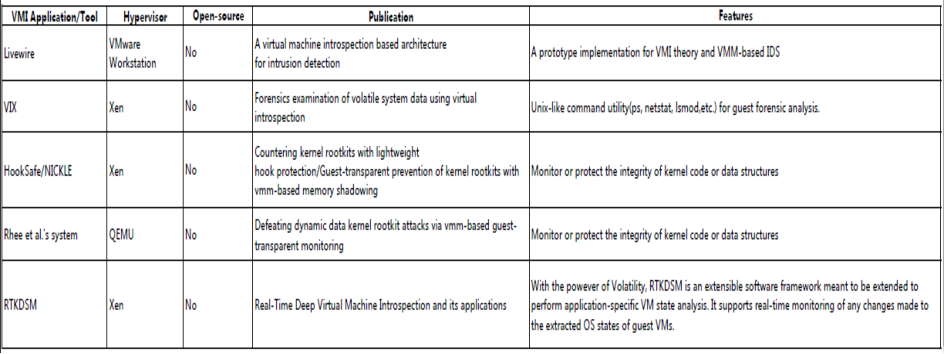
\includegraphics[scale=0.6]{Figures/Figure1.pdf}
	\caption[Out-of-Band pattern VMI applications]{Out-of-Band pattern VMI applications}
	\label{fig:Out-of-Band pattern VMI applications}
\end{figure}


\subsection{Derivative Pattern VMI APPLICATION}
Then we talk about some VMI applications based on derivative pattern. Manitou system use x6’s paging mechanism to perform integrity checks 
before code execution. From this work, we find paging mechanism is an important filed to explore to leverage derivative method. Antfarm is 
another typical example for derivative pattern. It is specially designed to monitor the VM’s memory management unit (MMU). From that, it could
construct the virtual-to-physical memory mapping and retrieve all running processes identified by a CR3 register value in guest. Lycosid allows
detecting and identifying all those hidden processes in guest. It first retrieves two different level process lists (cross-view validation) in 
guest by respectively using Antfarm and guest built-in utility (for example “ps” command in Linux/Unix world.). If number of processes contained
in these two different lists is not pertinent, Lycosid then infer the presence of some hidden processes and deduce those processes hidden by 
some statistical methods. Antfarm and Lycosid are both implemented in Xen platform and we have no access to its source code. However, these two
systems show a typical situation where we could apply derivative pattern. From these two applications, we also get to know that derivative 
pattern is really useful for security purpose, due to the fact that even though Lycosid is not familiar with the malicious process (PID, 
process name, etc.), it could interfere those dangerous activities.

Nitro, as far as I know, is the most recent derivate-pattern VMI application, whose objective is to trap system call events according to 
user-defined filter rule. For example, Nitro could be used as a technical building block retrieving all system calls for malware analysis. 
Due to its derivative pattern and open-source nature, Nitro is the focus of my investigation. Based on its functionality to access vCPU’s 
registers and system call trap, we intend to add network traffic monitoring functionality to Nitro and implement network monitoring on process 
granularity. However, Nitro is just under maintenance of Pfoh and has no updates since almost six months, even though it is an open-source 
project. Thus, there is not enough documentation about its utilization and it needs some enhancements besides its provided basic functionality.
Further introduction about Nitro are in the following part. All these derivative pattern VMI applications are summarized in Figure 
\ref{fig:Derivative pattern VMI applications}.

\begin{figure}[htbp]
	\centering
		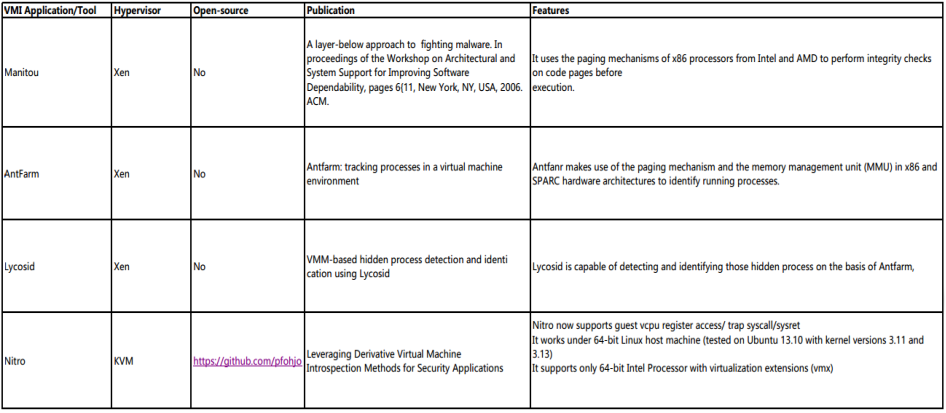
\includegraphics{Figures/Figure2.pdf}
	\caption[Derivative pattern VMI applications]{Derivative pattern VMI applications}
	\label{fig:Derivative pattern VMI applications}
\end{figure}



\section{VMI RELATED TOOLS}

Besides those mentioned VMI applications, we then talk about some interesting VMI Tools. These tools themselves are not VMI applications aiming
for certain security problems. Instead they may be in form of C library providing general VMI functionalities or forensic analysis frameworks 
to help bridge the semantic gap.

\subsection{LibVMI/XenAccess  \cite{Reference10,Reference11}}

LibVMI is an introspection library focused on reading and writing memory from running virtual machines. For convenience, LibVMI also provides 
functions for accessing CPU registers, pausing and unpausing a VM, printing binary data, and more. LibVMI is designed to work across multiple 
virtualization platforms. LibVMI currently supports VMs running in either Xen or KVM. LibVMI also supports reading physical memory snapshots 
when saved as a file.

XenAccess is predecessor of LibVMI but is focused exclusively on Xen. LibVMI is designed to work across a variety of virtualization platforms
including Xen and KVM. LibVMI provides a more intuitive API and therefore is more advised compared to XenAccess. Please refer to the following
link for more information: https://code.google.com/p/vmitools/. 

\subsection{Volatility  \cite{Reference13}}

The Volatility is an excellent open-source forensic analysis framework implemented in Python. It presents the advantage of bridging the 
semantic gap regardless of the system being monitored. Volatility has a wide range memory dump support, from Windows to Linux, from Mac OS
to Android. Also, there exist plenty of tutorials about this framework. Thus, recent years have witnessed increasing adoption of Volatility
in VMI application development, for example RTKDSM system. For more information, refer to this link: https://code.google.com/p/volatility/.

\subsection{Insight-VMI  \cite{Reference14,Reference15}}

Similar to Volatility, Insight-VMI is another open-source forensic analysis framework written in C++. Compared to Volatility, it additionally
provides an interactive shell for manual analysis of kernel objects and a JavaScript engine for automated analysis of repeating or complex 
tasks, but it now supports only Linux memory analysis. In addition, Insight-VMI and Nitro are both developed and maintained by the same study
team at the Technische Universität München in Germany. Detailed information is available in: https://code.google.com/p/insight-vmi/.

\begin{figure}[htbp]
	\centering
		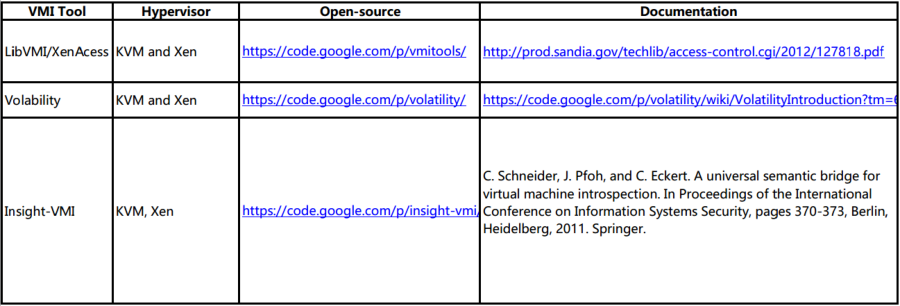
\includegraphics{Figures/Figure3.pdf}
		\rule{5em}{0.5pt}
	\caption[VMI Tool manifest]{VMI Tool manifest}
	\label{fig:VMI Tool manifest}
\end{figure} 
% Chapter Template

\chapter{INTERNSHIP’S OBJECTIVE} % Main chapter title

\label{Chapter3} % Change X to a consecutive number; for referencing this chapter elsewhere, use \ref{ChapterX}

\lhead{Chapter 3. \emph{INTERNSHIP’S OBJECTIVE}} % Change X to a consecutive number; this is for the header on each page - perhaps a shortened title

As mentioned before, in terms of bridging semantic gap for VMI, the most popular method is out-of-band delivery pattern. In this field, there exist plenty of VMI applications for various purposes. Although this method could help to effectively mitigate the semantic gap, it poses other problems such as portability, non-robust against circumstances technologies, etc. For example, if we use LibVMI to help parse guest Linux kernel data structure, the system symbol file is required firstly to be transferred to host machine. In case of kernel’s update in guest, this file transfer needs to be executed again. In this context, we want to explore the potential of derivative pattern, which relies on guest hardware architecture to extract useful information. Pfoh has declared in his work \citep{Reference7} that:

\textcolor{blue}{“These methods allow one to enumerate the running processes, monitor system calls, or track network connections on a per-process basis in a completely guest OS agnostic manner.” }

His declaration is rather interesting and attractive even though Pfoh has not given more explanation to argue his idea. Thus, the main objective of this internship is to prove this idea and develop a prototype implementation. The prototype should present the following features:

\begin{itemize}
    \item Capable of tracking network connection on a per-process
    \item Works in derivative method and independent of guest OS
 \end{itemize}

In conclusion, it’s a “netstat-like” utility by leveraging derivative pattern to bridge semantic gap and works out of monitored guest.

We plan to achieve our determined goal by the following steps:

\begin{itemize}
    \item Install and manipulate Nitro to see how derivative pattern works
    \item Study which component in KVM virtualization platform is in charge of virtual networking
    \item Study how to enumerate running process in a guest agnostic manner
    \item Study how to correlate each network connection with identified running process 
 \end{itemize}

% Chapter Template

\chapter{STUDY OF VMWALL\citep{Reference2}} % Main chapter title

\label{Chapter4} % Change X to a consecutive number; for referencing this chapter elsewhere, use \ref{ChapterX}

\lhead{Chapter X. \emph{STUDY OF VMWALL}} % Change X to a consecutive number; this is for the header on each page - perhaps a shortened title

Our strategy to achieve our goal is firstly to absorb inspiration from already-existing VMI applications. Among all the
VMI applications that we have studied, VMWall is relatively much closer to our design goal. This system implements
an application-level firewall working in Xen hypervisor. To achieve this, it needs to correlate each monitored TCP or
UDP connection with process which creates it. Although VMWall is implemented in Xen hypervisor and its source code
is not accessible, its work about how to correlate network traffic and corresponding process may give us some clues.

VMWall consists of two parts: user agent and kernel component. Kernel component uses a modified ebtables [21]
packet filter to intercept all packets sent to or from a guest domain. To well understand VMWall’s kernel component
implementation, it is supposed to be familiar with Xen network virtualization. In fact, Xen offers several different
9networking modes. VMWall uniquely considers the bridging mode. With this mode, Dom0 provides a virtual Ethernet
bridge connecting the physical network card to all virtual network devices provided by Xen to the domU VMs. Dom0
uses its virtual bridge to multiplex and demultiplex packets between the physical network interface and each
unprivileged virtual machine’s VNI (Virtual Network Interface). Due to this fact mentioned, kernel component (in this
case Ebtables) could intercept all packets between monitored VM and external Internet and retrieve information like IP
address and TCP/UPD port to identify a network connection.

If necessary, user agent, another important part of VMWall, will receive a request containing IP address and TCP ports
information and need to use the latter to identify the corresponding process running in monitored guest by out-of-band
pattern VMI. The correlation between network connection and process relies on one file type in Linux/Unix: socket.
Socket is a special file type in Linux/Unix world. To create a socket connection, IP address and transport layer port are
required. All opening port numbers in Linux are hashed and managed by data structure \lq inet\_hashinfo \rq. By iterating this
variable (for example tcp\_hashinfo) of this data structure, the socket file using a given port number could be identified. Similarly, all processes in Linux are managed by a double linked data structure \lq task\_struct \rq. With input of a certain socket reference, the process creating this socket could be found. The following picture shows how to correlate network
connection and process on data structure level.

\begin{figure}[htbp]
	\centering
		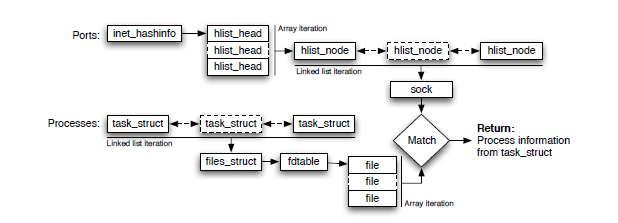
\includegraphics[scale = 0.8 ]{Figures/Figure4.png}
		% \rule{35em}{0.5pt}
	\caption[Out-of-Band pattern VMI applications]{Out-of-Band pattern VMI applications}
	\label{fig:Guest Linux kernel data structures traversed by the VMWall user agent during correlation of the
process and TCP packet information}
\end{figure}

%----------------------------------------------------------------------------------------
%	SECTION 1
%----------------------------------------------------------------------------------------

\section{Main Section 1}

Lorem ipsum dolor sit amet, consectetur adipiscing elit. Aliquam ultricies lacinia euismod. Nam tempus risus in dolor rhoncus in interdum enim tincidunt. Donec vel nunc neque. In condimentum ullamcorper quam non consequat. Fusce sagittis tempor feugiat. Fusce magna erat, molestie eu convallis ut, tempus sed arcu. Quisque molestie, ante a tincidunt ullamcorper, sapien enim dignissim lacus, in semper nibh erat lobortis purus. Integer dapibus ligula ac risus convallis pellentesque.

%-----------------------------------
%	SUBSECTION 1
%-----------------------------------
\subsection{Subsection 1}

Nunc posuere quam at lectus tristique eu ultrices augue venenatis. Vestibulum ante ipsum primis in faucibus orci luctus et ultrices posuere cubilia Curae; Aliquam erat volutpat. Vivamus sodales tortor eget quam adipiscing in vulputate ante ullamcorper. Sed eros ante, lacinia et sollicitudin et, aliquam sit amet augue. In hac habitasse platea dictumst.

%-----------------------------------
%	SUBSECTION 2
%-----------------------------------

\subsection{Subsection 2}
Morbi rutrum odio eget arcu adipiscing sodales. Aenean et purus a est pulvinar pellentesque. Cras in elit neque, quis varius elit. Phasellus fringilla, nibh eu tempus venenatis, dolor elit posuere quam, quis adipiscing urna leo nec orci. Sed nec nulla auctor odio aliquet consequat. Ut nec nulla in ante ullamcorper aliquam at sed dolor. Phasellus fermentum magna in augue gravida cursus. Cras sed pretium lorem. Pellentesque eget ornare odio. Proin accumsan, massa viverra cursus pharetra, ipsum nisi lobortis velit, a malesuada dolor lorem eu neque.

%----------------------------------------------------------------------------------------
%	SECTION 2
%----------------------------------------------------------------------------------------

\section{Main Section 2}

Sed ullamcorper quam eu nisl interdum at interdum enim egestas. Aliquam placerat justo sed lectus lobortis ut porta nisl porttitor. Vestibulum mi dolor, lacinia molestie gravida at, tempus vitae ligula. Donec eget quam sapien, in viverra eros. Donec pellentesque justo a massa fringilla non vestibulum metus vestibulum. Vestibulum in orci quis felis tempor lacinia. Vivamus ornare ultrices facilisis. Ut hendrerit volutpat vulputate. Morbi condimentum venenatis augue, id porta ipsum vulputate in. Curabitur luctus tempus justo. Vestibulum risus lectus, adipiscing nec condimentum quis, condimentum nec nisl. Aliquam dictum sagittis velit sed iaculis. Morbi tristique augue sit amet nulla pulvinar id facilisis ligula mollis. Nam elit libero, tincidunt ut aliquam at, molestie in quam. Aenean rhoncus vehicula hendrerit. 
% Chapter Template

\chapter{ESTABLISHMENT OF EXPERIMENTATION PLATFORM} % Main chapter title

\label{Chapter5} % Change X to a consecutive number; for referencing this chapter elsewhere, use \ref{ChapterX}

\lhead{Chapter 5. \emph{ESTABLISHMENT OF EXPERIMENTATION PLATFORM}} % Change X to a consecutive number; this is for the header on each page - perhaps a shortened title

As the state-of-the-are about VMI is finished and the objective is determined, we plan to implement a prototype in
KVM virtualization platform. With a HP workstation at disposal, we need firstly to establish an experimentation and
development platform.

%----------------------------------------------------------------------------------------
%	SECTION 1
%----------------------------------------------------------------------------------------

\section{WIN7 and UBUNTU DUAL-BOOT SYSTEM}

As was mentioned above, the first step to achieve our final objective is to figure out how derivative pattern functions by
installing and manipulating the only known open-source derivative pattern VMI application: Nitro. Thus, it’s logical to
choose those operating systems which support Nitro. According to Pfoh, Nitro has been tested on Linux kernel 3.11 and
3.13. Hence, Ubuntu14.04 with kernel version 3.13 is our final choice.
KVM virtualization platform will be built in a HP Z820 workstation which initially has only Windows 7 installed. The
first step is to install a Windows 7 and Ubuntu 14.04 dual-boot system. This manipulation is not difficult but kind of
tedious. In fact, we follow this tutorial http://askubuntu.com/questions/343268/how-to-use-manual-partitioning-during-
installation to accomplish this step.

%-----------------------------------
%	SUBSECTION 2
%-----------------------------------

\section{NETWORK CONFIGURATION}

This workstation has been allocated a static network configuration and it uses always port 8 in each office. To achieve
this, we need to edit configuration file /etc/network/interfaces to set 10.193.192.37 as ipv4 address, 255.255.255.0 as
10network mask, 10.193.192.1 as default gateway and 10.193.197.10 as DNS name server. The final network configuration in 
Ubuntu14.04 is shown as following.

\begin{figure}[htbp]
	\centering
		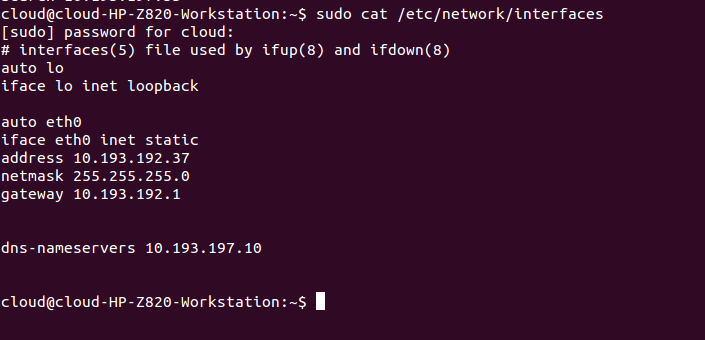
\includegraphics[scale = 0.8]{Figures/Figure5.png}
	\caption[HP Workstation static network configuration]{HP Workstation static network configuration}
	\label{fig:HP Workstation static network configuration}
\end{figure}

Besides, never forget to set a parameter named “managed” to “true”, defined in configuration file /etc/NetworkManager/NetworkManager.conf. 
Otherwise the network will be always in disable state. The security politics of Orange Labs require each PC to configure proxy server if the former needs Internet connectivity.
In fact, under Linux system, it is possible to set proxy configuration on different level. The first solution is to declare http proxy server on command-line level. 
For example, if we want to update APT source list, we could issue a command in a terminal:
sudo http://proxy.rd.francetelecom.fr:8080 apt-get update
This proxy configuration is uniquely valid for the current command and every command we tape should contain an option for proxy server, which is not effective and tedious.
Proxy server configuration could also be set on application level. For example, if we want to user web browser such as Firefox, 
we need to set proxy address for Firefox just like in the following picture.

\begin{figure}[htbp]
	\centering
		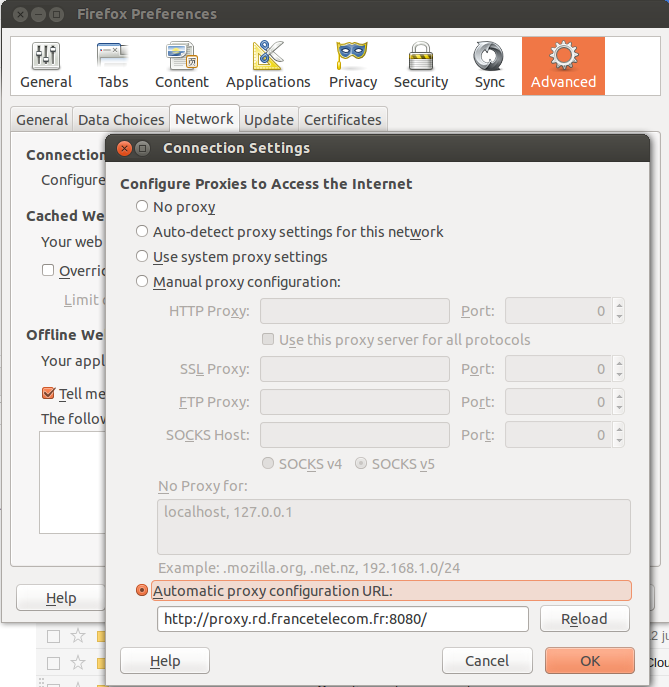
\includegraphics[width=12cm, height= 9cm ]{Figures/Figure6.png}
	\caption[Firefox proxy parameter]{Firefox proxy parameter}
	\label{fig:Firefox proxy parameter}
\end{figure}

To use APT command to install software, we need to edit (if not exist, create) a configure file named \lq apt.conf \rq under /etc/apt. This file just contains one line: Acquire::http::proxy::”http://proxy.rd.francetelecom.fr:8080”
Then we could issue command like \lq sudo apt-get install software\_name \lq as normal in terminal. In one word, it is supposed to configure proxy server address for every application which needs Internet connectivity.
The last solution is setting bash configuration files like /etc/profile, /etc/bash.bashrc or ~/.bashrc. Proxy configuration in this manner is user or all-user level. Only once configuration is needed to guarantee Internet connectivity for all applications.


%----------------------------------------------------------------------------------------
%	SECTION 3
%----------------------------------------------------------------------------------------
\section{KVM Introduction}

After installation of Ubuntu14.04 in our workstation, it’s time to install required Ubuntu packages to turn Ubuntu into a hypervisor. Prior to the real installation, it is necessary to make a presentation for KVM.

KVM (Kernel-based Virtual Machine) is a virtualization infrastructure for the Linux kernel that turns it into a hypervisor, which was merged into the Linux kernel mainline in February 2007. KVM requires a processor with hardware virtualization extension. KVM has also been ported to FreeBSD and Illumos in the form of loadable kernel modules. 
Compared to other virtualization alternatives available in Linux, KVM presents the following advantages \citep{Reference20}:

    \begin{itemize}
	\item Can interact directly with the Kernel
	\item Default virtualization in leading Linux Distributions
	\item One of the Linux software developed aggressively.
	\item Almost becoming competitor to VMware by implementing technologies such as v2v, p2v, and many open source tools to manage VM
	\item Number of open source cloud automation softwares use KVM as default hypervisor 

    \end{itemize}

%----------------------------------------------------------------------------------------
%	SECTION 4
%----------------------------------------------------------------------------------------

\section{KVM’s Operating Principle}

Once KVM is installed on a Linux box, a hardware file /dev/kvm is created which will act as interpreter between actual hardware and hypervisor manager (for example, virt-manager). 
Whenever a request for hardware changes or additions comes from hypervisor manager, KVM software starts allocating those resources virtually by interacting with real hardware. 
Suppose we want to change RAM on a virtual machine, this is communicated by the hypervisor manager to KVM for allocating the resource. 
Then KVM interacts with hardware and reserves that RAM from real RAM for that particular VM. This happens for the other resources as well.

\begin{figure}[htbp]
	\centering
		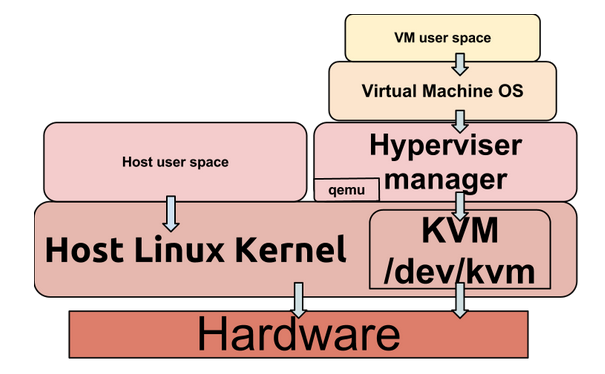
\includegraphics[scale = 0.6]{Figures/Figure7.png}
	\caption[KVM Virtualization Architecture in Linux]{KVM Virtualization Architecture in Linux}
	\label{fig:KVM Virtualization Architecture in Linux}
\end{figure}


\section{KVM’s VM Management Tools}

There exists several methods in KVM for management activity such as guest’s creation, deletion, start, stop and clone,etc.

\subsection{virt-manager}
The most popular GUI is called Virtual Machine Manager (VMM), developed by RedHat. 
The tool is also known by its generic package name virt-manager. 
It comes with a number of supporting tools, including virt-install, virt-clone, virt-image, and virt-viewer, 
which are used to provision, clone, install, and view virtual machines, respectively. 
VMM also supports Xen machines. Virt-manager relies on libvirt and uses qemu to run guest instance. 
In the following section, we will show how to create a KVM guest with virt-manager.

\subsection{virsh}
The generic KVM command interface is provided by virsh. virsh is a shell for managing hypervisors and VM’s directly from host OS terminal. 
Specifically, you can use the supporting tools, like virt-install for creating your virtual machines. 
On Ubuntu, there's a special ubuntu-vm-builder tool that can be used for provisioning Ubuntu builds, developed by Canonical.

\subsection{qemu command line with ''enable-kvm'' option}
In fact, virt-manager or virsh both could be regarded as wrapper based on libvirt and qemu. 
As a result, we could use qemu command lines to manage KVM guests with “enable-kvm” option to profit performance acceleration offered by KVM. 
However, this method is not handy compared to virt-manager and virsh. 
Note that Nitro is only able to monitor KVM guests launched by a modified version qemu. 
We could use GUI tools such as virt-manager to create virtual machines images and issue qemu command line to start created VM and start Nitro to monitor these VMs.

\subsection{KVM command}
KVM also has its own syntax, similar to QEMU. 
It is not a recommended way of managing virtual machines. 
More information is available with link: https://help.ubuntu.com/community/KVM/Directly

\subsection{Libvirt}
Libvirt is not a VM management tool. 
Instead, it is a toolkit to interact with the virtualization capabilities of recent versions of Linux \citep{Reference23}. 
It is an open-source project and provides a set of long term stable C API. 
These C APIs all APIs are designed to do virtualization management, such as: 
provision, create, modify, monitor, control, migrate and stop the guests - within the limits of the support of the hypervisor for those operations. 
Hence, libvirt is intended to be a building block for higher level management tools and for applications focusing on virtualization of a single physical host. 
The following picture shows the relationship between hypervisor, libvirt and virtualization management tool.

\begin{figure}[htbp]
	\centering
		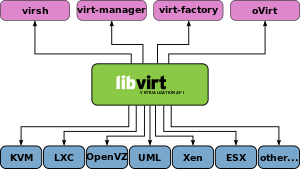
\includegraphics[scale = 1.2]{Figures/Figure8.png}
	\caption[Relationship between virsh, virt-manager and libvirt]{Relationship between virsh, virt-manager and libvirt}
	\label{fig:Relationship between virsh, virt-manager and libvirt}
\end{figure}

\section{KVM/QEMU networking}
Guest (VM) networking in KVM is the same as in qemu, 
so it is possible to refer to other documentations about networking for qemu. 
In this section, we will talk about the three most frequent types of network needed.
\subsection{User Networking}
This networking mode, shown in figure \ref{fig:User networking mode topology}, allows guests accessing to the host, to the internet. 
However, the guests are neither invisible from outside network nor from other VMs. 
In addition, user networking does not support other network protocols other than TCP/UDP. 
Hence, certain applications (like ping) won't work.

\begin{figure}[htb]
	\centering
		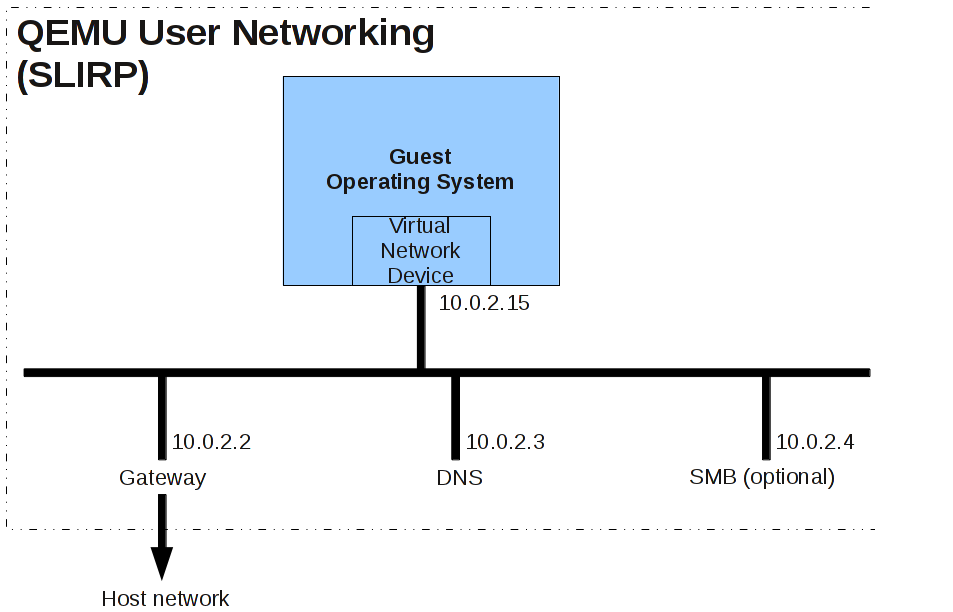
\includegraphics[scale=0.5]{Figures/Figure9.png}
	\caption[User networking mode topology]{User networking mode topology}
	\label{fig:User networking mode topology}
\end{figure}

For example, we could issue the following to start a guest in user networking mode:
\shellcmd{qemu-system-x86\_64 -enable-kvm -had win7.img -m 2048}
The guest OS will see an E1000 NIC with a virtual DHCP server on 10.0.2.2 and will be 
allocated an address starting from 10.0.2.15. A virtual DNS server will be accessible on 10.0.2.3.

\subsection{Bridged Networking}
The bridge networking mode makes all launched guests run just like they are in the same local network with host machine.  
To use bridged networking, a virtual Ethernet bridge should be firstly created. Under Ubunu14.04, 
we need to edit /etc/network/interfaces as following, for example:

\# The content of file /etc/network/interfaces\\
\# Replace old eth0 config with br0, there no more "auto eth0" \\
auto br0\\
\# Use old eth0 config for br0, plus bridge stuff\\
iface br0 inet static\\
	\indent\indent \# Attention use old static configuration of eth0\\
	\indent\indent bridge\_ports    eth0\\
	\indent\indent bridge\_stp      off\\
	\indent\indent bridge\_maxwait  0\\
	\indent\indent bridge\_fd       0\\
	
Run each guest with the following, replacing \$macaddress with a customized MAC address.
\shellcmd{qemu-system-x86\_64 -hda /path/to/hda.img -device e1000,netdev=net0,mac=\$macaddress-netdev tap,id=net0}

\subsection{networking mode}
NAT networking mode is actually the default networking mode for virtual machines created by virt-manager.
\begin{figure}[htb]
	\centering
		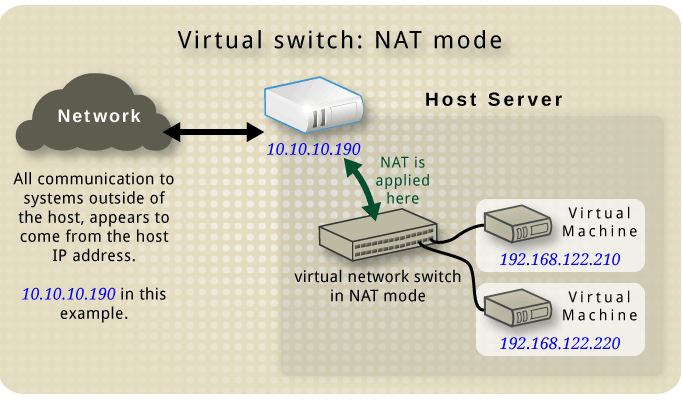
\includegraphics[scale=0.5]{Figures/Figure10.png}
	\caption[Virtual network on NAT mode]{Virtual network on NAT mode}
	\label{fig:Virtual network on NAT mode}
\end{figure}


\section{KVM installation}
KVM is a virtualization feature in the Linux kernel that lets a program like qemu safely execute guest code directly on the host CPU. 
This is only possible when the target architecture is supported by the host CPU. 
CPU’s virtualization extension (VMX for Intel’s processors and SVM for AMD.) support could be verified by issuing this following command in a terminal:
\shellcmd{ grep -c '(vmx|svm)' /proc/cpuinfo }
A return value greater than zero means that current CPU supports KVM. In addition, it’s necessary to check virtualization technology is enabled in BIOS. 
After enabling this feature, we have to cold power-cycle the machine for the change to take effect. 
Once this is done, run kvm-ok to verify:  
\begin{figure}[htbp]
	\centering
		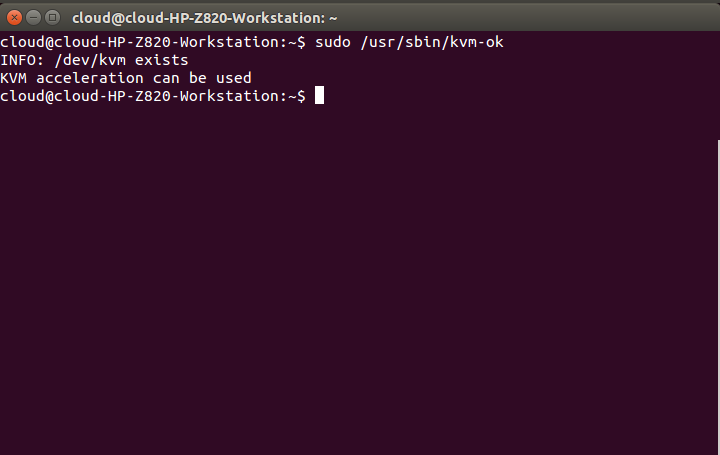
\includegraphics[scale=0.7]{Figures/Figure11.png}
	\caption[Output of kvm-ok command]{Output of kvm-ok command}
	\label{fig:Output of kvm-ok command}
\end{figure}

Then we begin to install required packages for KVM. The command to install everything you need is:
\shellcmd{ sudo apt-get install qemu-kvm libvirt-bin ubuntu-vm-builder bridge-utils}
\shellcmd{ sudo apt-get install virt-manager virtinst qemu-system}
Out of interest, KVM doesn’t have its own configuration directory. The configuration files could be found in: /etc/libvirt/qemu/
There are some quirks or confusions which deserve clarify, in term of difference and association between libvirt, 
qemu, qemu-kvm. Qemu in fact is project independent of KVM, it is an emulator which itself could be used as a virtualization 
alternative. Qemu-kvm is fork of QEMU maintained by KVM project. Currently (close to the 1.1 release) it still provides the best 
performance and certain additional features for using KVM with QEMU on x86. Any other architecture is already fully supported by QEMU itself. However QEMU development community plans to suspend the development of qemu-kvm and make qemu master fork to support all architectures. Libvirt is a toolkit to interact with the virtualization capabilities of recent versions of Linux [23]. It is an open-source project and provides a set of long term stable C API. These C APIs all APIs are designed to do virtualization management, such as: provision, create, modify, monitor, control, migrate and stop the guests - within the limits of the support of the hypervisor for those operations. Hence, libvirt is intended to be a building block for higher level management tools and for applications focusing on virtualization of a single physical host. The following picture shows the relationship between hypervisor, libvirt and virtualization management tool. 

\section{KVM Win7 Guest Manipulation} 
After establishing KVM virtualization platform, we plan to create a Windows 7 64 bits guest with virt-manager. 
To launch virt-manager, open a terminal and issue the following command: 
\shellcmd{ sudo virt-manager}
We name this guest as ``win7\_64bit'', chose a local installation place then click forward button.
\begin{figure}[htbp]
	\centering
		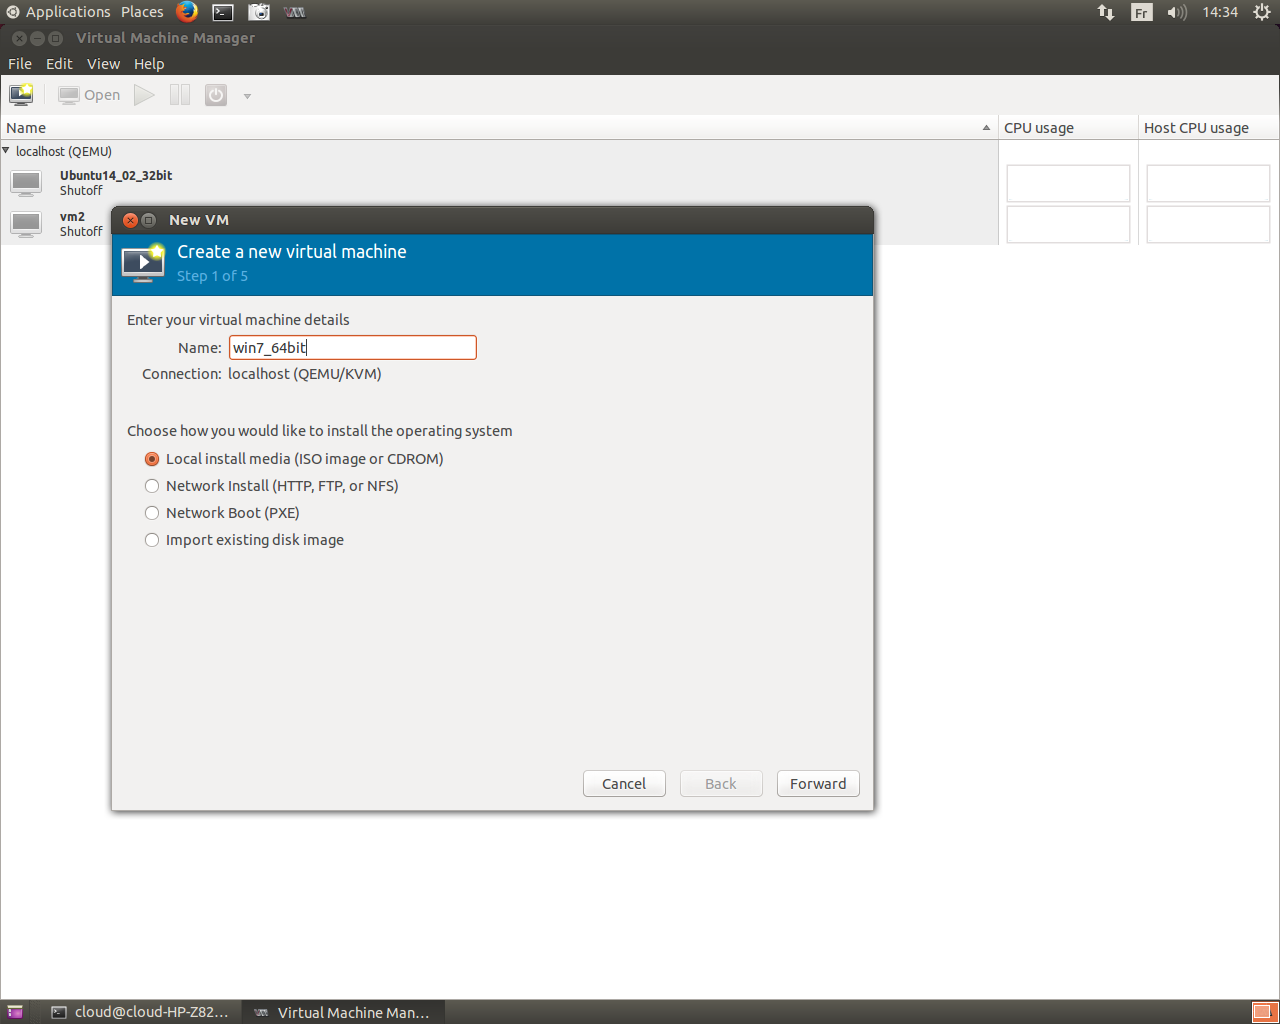
\includegraphics[scale=0.4]{Figures/Figure12.png}
	\caption[Step 1-Create a new VM with name win7\_64bit]{Step 1-Create a new VM with name win7\_64bit}
	\label{fig:Step 1-Create a new VM with name win7-64bit}
\end{figure}

At step 2 shown in Figure \ref{fig:Choose win7 ISO file}, we need to indicate the location of the win7 installation ISO file for virt-manager.
\begin{figure}[htbp]
	\centering
		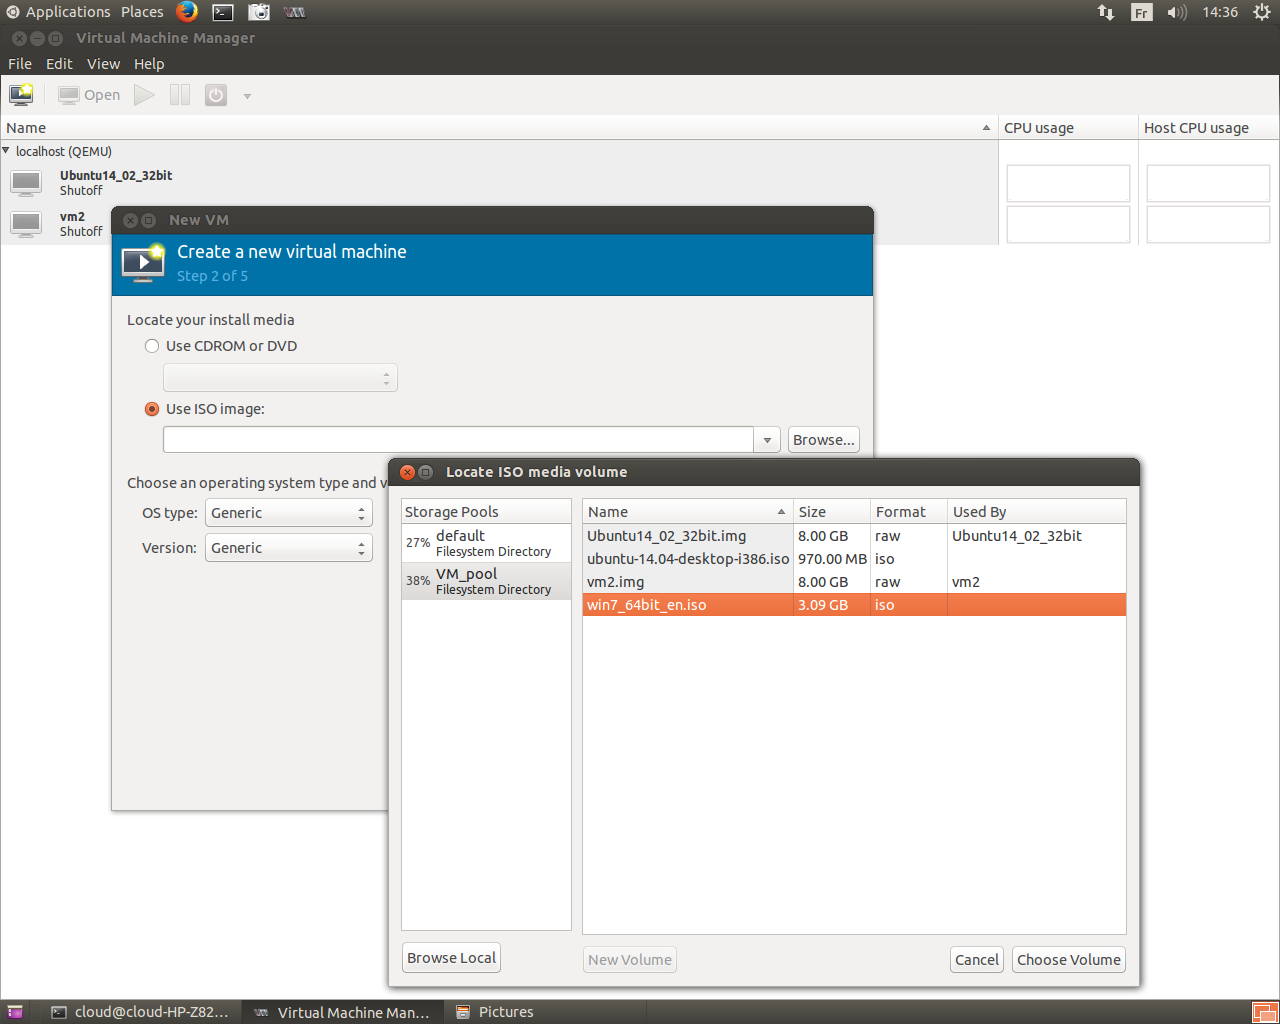
\includegraphics[scale=0.4]{Figures/Figure13.png}
	\caption[Step 2-Choose win7 ISO file]{Step 2-Choose win7 ISO file}
	\label{fig:Choose win7 ISO file}
\end{figure}

Then we create a virtual disk of 20G for our guest in step 3 (Figure \ref{fig:Step 3-Create a virtual disk of 20G}).
\begin{figure}[htbp]
	\centering
		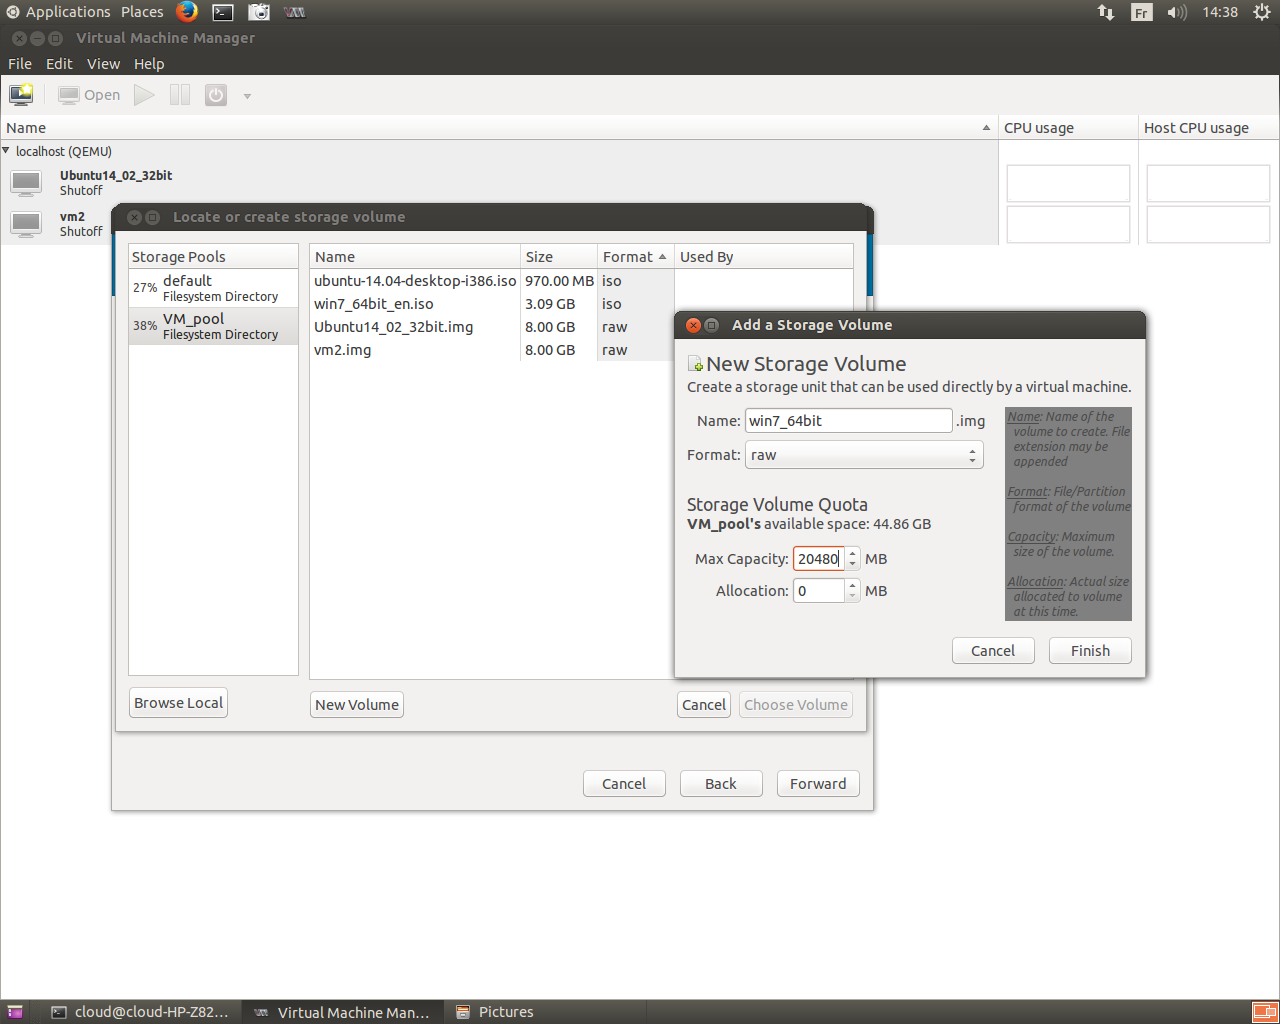
\includegraphics[scale=0.4]{Figures/Figure14.png}
	\caption[Step 3-Create a virtual disk of 20G]{Step 3-Create a virtual disk of 20G}
	\label{fig:Step 3-Create a virtual disk of 20G}
\end{figure}

In the next step (Figure \ref{fig:Step 4-Indicate virtual disk location for guest installation}), our reserved virtual disk is used as hard disk for win7\_64bit guest.
\begin{figure}[htbp]
	\centering
		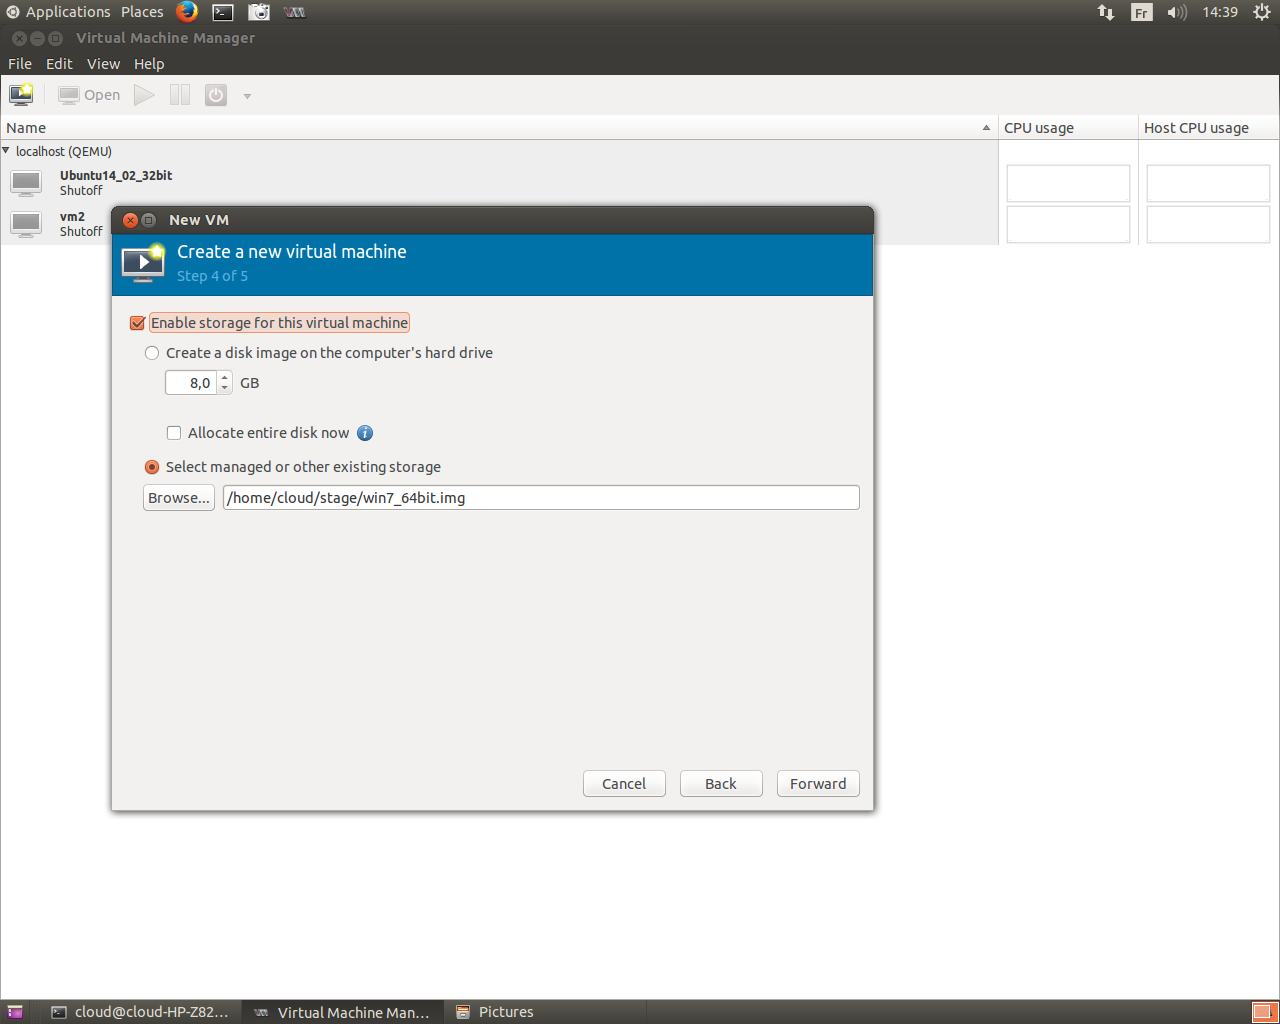
\includegraphics[scale=0.4]{Figures/Figure15.png}
	\caption[Step 4-Indicate virtual disk location for guest installation]{Step 4-Indicate virtual disk location for guest installation}
	\label{fig:Step 4-Indicate virtual disk location for guest installation}
\end{figure}

The last step (Figure \ref {fig:Step 5-Guest installation configuration resume}) is a resume of installation configuration. Note that the guest works with NAT network mode.
\begin{figure}[htbp]
	\centering
		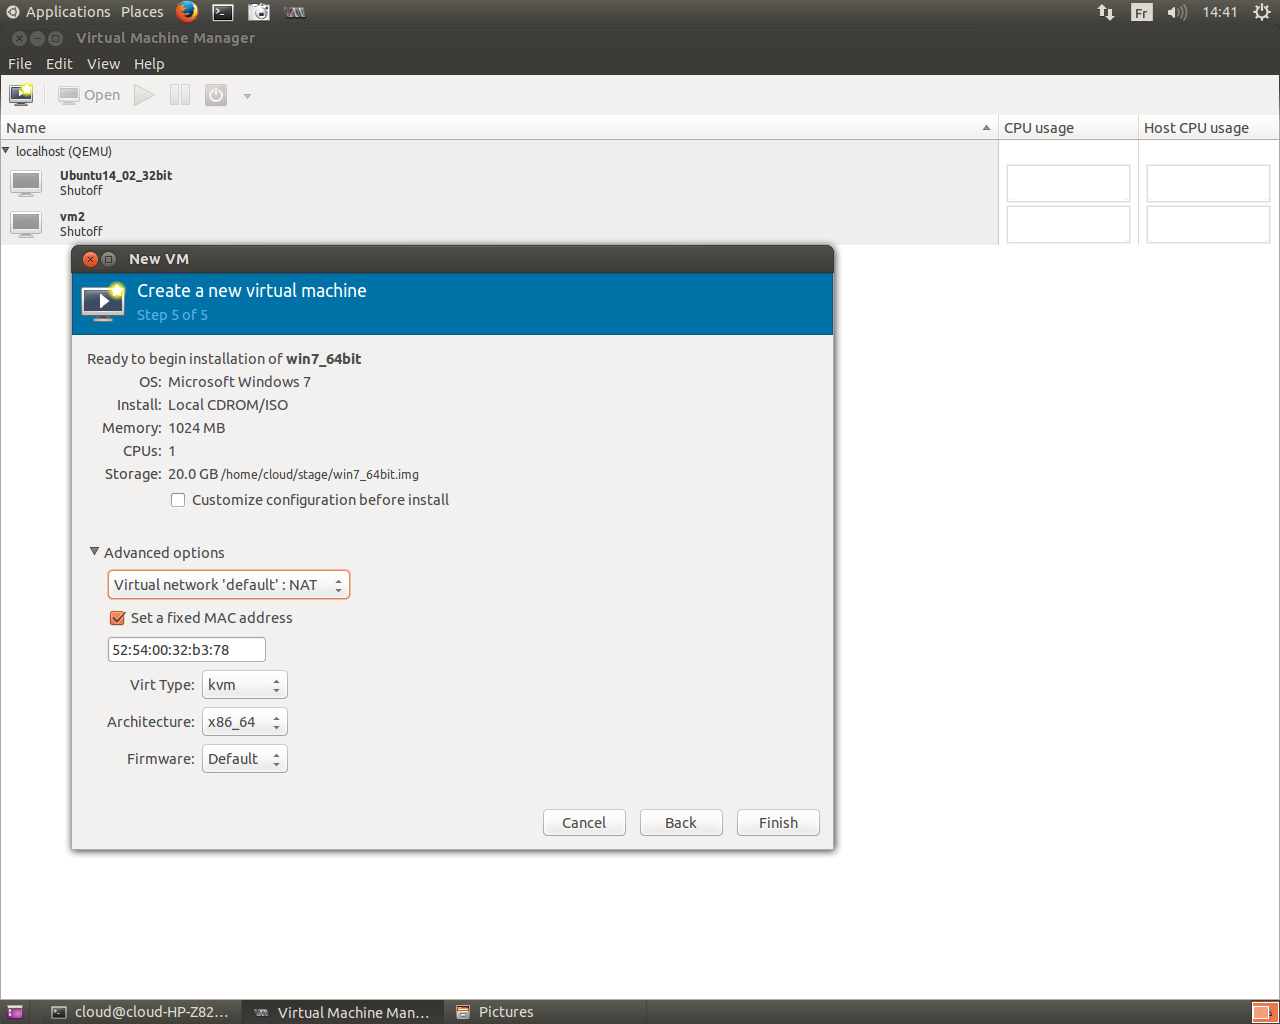
\includegraphics[scale=0.4]{Figures/Figure16.png}
	\caption[Step 5-Guest installation configuration resume]{Step 5-Guest installation configuration resume}
	\label{fig:Step 5-Guest installation configuration resume}
\end{figure}

When the installation process is finished, we check guest’s IP configuration and ping the host. The result is shown in picture \ref{fig:guest machine ping host machine}.
\begin{figure}[htbp]
	\centering
		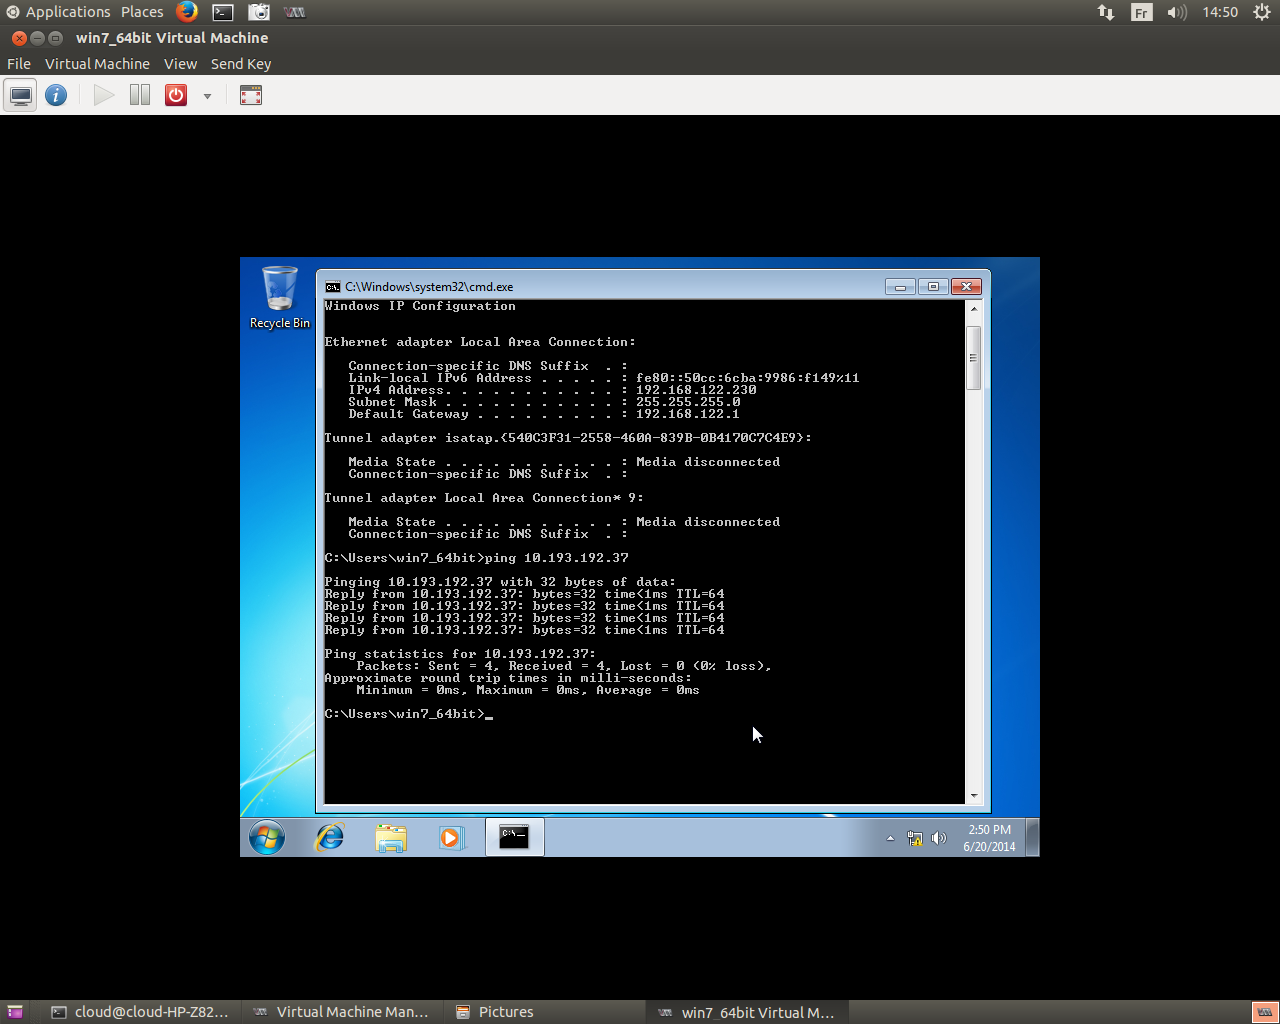
\includegraphics[scale=0.4]{Figures/Figure17.png}
	\caption[Guest machine ping host machine]{Guest machine ping host machine}
	\label{fig:guest machine ping host machine}
\end{figure}

Then verify that the guest machine is launched as a seperate process under Ubuntu by qemu in host machine. The result is shown in Figure \ref{fig:Guest as a qemu process in host machine}
\begin{figure}[htbp]
	\centering
		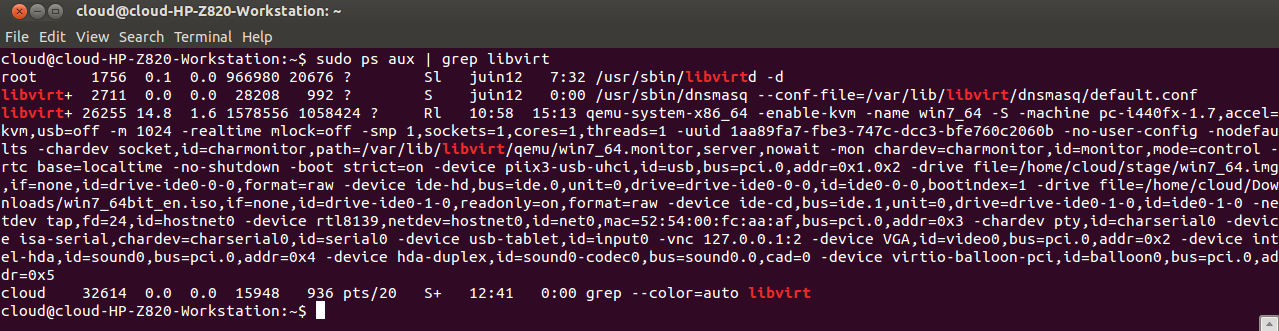
\includegraphics[width=14cm, height= 4cm ]{Figures/Figure18.png}
	\caption[Guest as a qemu process in host machine]{Guest as a qemu process in host machine}
	\label{fig:Guest as a qemu process in host machine}
\end{figure}


 
% Chapter Template

\chapter{Nitro installation and manipulation} % Main chapter title

\label{Chapter6} % Change X to a consecutive number; for referencing this chapter elsewhere, use \ref{ChapterX}

\lhead{Chapter 6. \emph{Nitro installation and manipulation}} % Change X to a consecutive number; this is for the header on each page - perhaps a shortened title

%----------------------------------------------------------------------------------------
%	SECTION 1
%----------------------------------------------------------------------------------------

\section{Installation of Nitro}

Pfoh has created a website, http://nitro.pfoh.net/setup.html, where he gives a general introduction about Nitro’s setup. To reduce the length of this report, it’s advised to carefully follow Pfoh’s tutorial when installing Nitro. Here we just provide some extra explanations and complements on the basis of his initial tutorial. Remember Nitro consists of three components:
\begin{itemize}
    \item Kernel Modules - This component is a fork of KVM. It has been extended to provide additional IOCTL calls that can be leveraged to perform VMI.
    \item QEMU - This is a fork of QEMU, the component that provides the user land support for KVM. It is only slightly modified such that it exposes direct access to the guest's physical memory, which Nitro can take advantage of.
    \item Nitro/libnitro - This is the user land component that actually performs VMI. Nitro (this term here represents an executable file/command as opposed to the Nitro project.) calls those APIs defined in libnitro. Remember Nitro is just a prototype implementation which still needs much more enhancements if you want more functionality and could be used as a technique block in other projects. To facilitate possible further work, we have added plenty of comments in Nitro’s source code files. We put Nitro’s source files in path /home/cloud/nitro.
\end{itemize}

%----------------------------------------------------------------------------------------
%	SECTION 2
%----------------------------------------------------------------------------------------

\section{Manipulation of Nitro}

To use Nitro, some preliminary work is necessary, including replace initial KVM modules by a modified one for Nitro, 
mount a huge pages type device under /tmp directory and finally increase the number of huge pages available to your system. 
If you are not familiar with huge pages, this tutorial is a good start point: https://wiki.debian.org/Hugepages. 
To automate this work, we have written a bash shell script named “load\_mods”, which is located in the root of working directory (/home/cloud/load\_mods). 
If not precise, all script files for Nitro are in the same location. 

Once the huge table file system is set up, QEMU could be launched. 
Note that Nitro uses a modified version of QEMU to directly access the guest's physical memory. 
We put this QEMU in the root of user cloud’s working directory (/home/cloud/qemu). 
When staring the modified QEMU, it works in the same manner as starting vanilla QEMU with KVM support, 
but you must include option “-mem-path [PATH] -mem-prealloc” in the end of QEMU command line. 
It is recommended to use a bash script to automate this work. For example, to start guest with WIN7 OS, 
we write a script named “win7start”.

Finally, it’s time to launch Nitro to monitor the already running VM. We have also a script “NitroStart” for this work. 
Note that Nitro command syntax is “./Nitro PID GUEST\_RAM\_FILE”. Figure \ref{fig:Truncated output of Nitro for a Win7 64bit VM} shows a part of output of Nitro.

\begin{figure}[htbp]
	\centering
		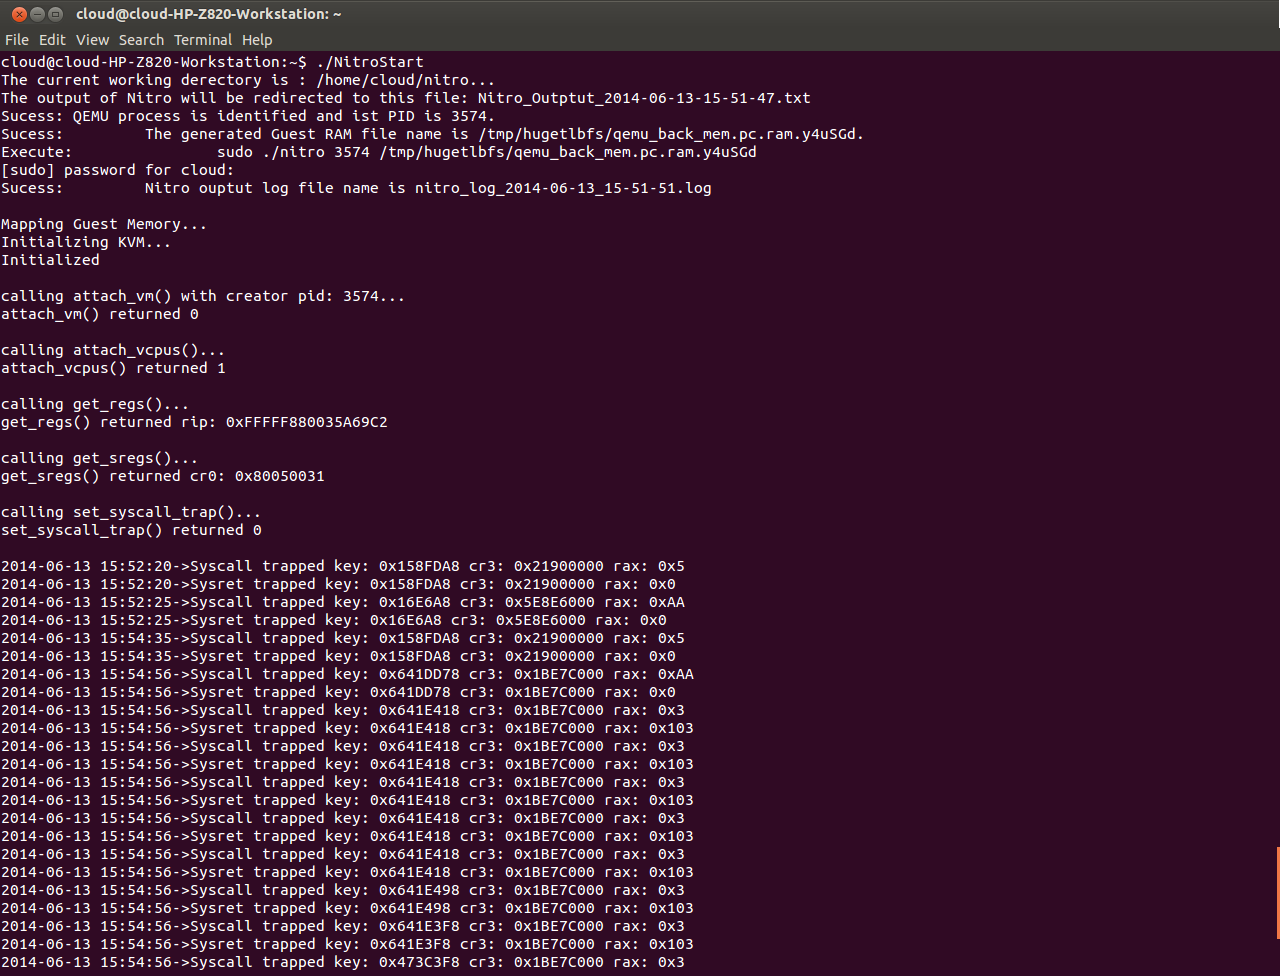
\includegraphics[width=14cm, height= 10cm ]{Figures/Figure19.png}
	\caption[Truncated output of Nitro for a Win7 64bit VM]{Truncated output of Nitro for a Win7 64bit VM}
	\label{fig:Truncated output of Nitro for a Win7 64bit VM}
\end{figure}

All the output of Nitro could be devised into two parties. 
The first part logs the Nitro start process and prints return values for each function invocation. 
For example, function attach\_vcpu( ) returns 1 if Nitro manages to attach to a virtual CPU in guest machine.
(In fact, Nitro now support uniquely attachment to one virtual CPU even if the guest has been allocated more than one virtual CPU.). 
When the invocation of set\_syscall\_trap() returns zero, Nitro is successfully started and ready to capture system call events.
The second part of this output consists of all trapped system call events. Column “Syscall trapped key” means the physical address of 
related system call service routine. Column “cr3” save the CR3 register’s value at the moment of system call trap. And column “rax” 
indicates the system call code for windows 64 bits operating system. For example, a value “AA” in RAX means a system call 
“NtCreateUserProcess” in windows 7. In fact, in the prototype implementation provided by Pfoh, the type of system call desired is 
hard coded in file “nitro\_main.c”. Nitro captures only those system calls that users require.  
For more information about windows 64 bits system call table, please refer to this link: http://j00ru.vexillium.org/ntapi\_64/.

\section{Assessment of Nitro}
As far as I know, Nitro is actually the first and only VMI application in derivative manner under KVM virtualization platform. 
Though VMI in derivative mode is perfectly against circumstance technique, the amount of information obtained is rather limited, 
due to the fact that derivation method principally just concerns and observes hardware-related running state (such as CR3 register, etc.)
\cite{Reference17}. Nitro, as a typical implementation under the guide of derivation method, is no different. Currently, Nitro is just able to access vCPU 
registers and trap system calls of type “syscall/sysret” (In fact, system call is possible to be invoked in other manners such as assembly instruction int 0x80.), 
even though Pfoh promises to enrich Nitro’s functionality list in his spare time.

Just as Pfoh has stated in his project website, Nitro at present has a relatively limited suit of functionalities compared with 
those VMI tools like LibVMI in out-of-band. Concretely, it presents the following limitations:
\begin{itemize}
    \item No documentation about use of Nitro, which is really painful for beginners
    \item No support for AMD CPUs
    \item No support for multi-core guests
    \item Only 64-bit windows guests are supported for now
    \item No cooperation with other tools like virsh/virt-manager
\end{itemize}

The final conclusion for Nitro is that, as a prototype implementation for VMI derivative pattern theory, 
it is a good start point to study, manipulate and modify for the purpose of study, For example, 
to anatomy its modification about KVM modules, we could learn how to enhance KVM virtualization support. As a development framework, 
it is not enough mature to simplify development work, due to the fact Nitro itself is still a project in progress.

The above conclusion could be extended to a conclusion for derivative pattern for VMI application. 
Inferring information from hardware architecture to mitigate semantic gap, this pattern ignores OS-related semantic knowledge to 
get a better portability feature. However, to get high-level information, to implement monitoring task for example, OS-related semantic 
knowledge is somewhat indispensable. We suggest that:

\begin{itemize}
    \item Derivative pattern could be used alongside with Out-of-band pattern to provide a complementary view for guest running state
    \item Derivative is suitable to be used as the last defense line for security purpose
\end{itemize}


 
% Chapter Template

\chapter{LibVMI\&Volatility MANIPULATION} % Main chapter title

\label{Chapter7} % Change X to a consecutive number; for referencing this chapter elsewhere, use \ref{ChapterX}

\lhead{Chapter 7. \emph{LibVMI\&Volatility Manipulation}} % Change X to a consecutive number; this is for the header on each page - perhaps a shortened title

%----------------------------------------------------------------------------------------
%	SECTION 1
%----------------------------------------------------------------------------------------

\section{INTRODCTION}
Recall that the objective of this internship derives from a predication made by Pfoh in his doctoral thesis in chapter 6 
Derivative Method \cite{Reference7}: These methods (Derivative method) allow one to track network connections on a per-process
basis in a completely guest operating system agnostic manner.

Frankly, a Virtual Machine Introspection application VMWall \cite{Reference2} has implemented almost the similar functionality. 
However, VMWall’s implementation is based on delivery pattern, thus it has a narrow set of operating system support and requires
some preliminary configuration files to work. All above characteristics hinder wide application of this kind of VMI application.
Therefore, what Pfoh has declared actually attract my attention is the capacity presented by his derivative method to achieve
the same functionality but in a “completely guest operating system agnostic manner”.

To implement his claim, this task could be naturally treated from two plans: network plan and process plan. 
With regard to network plan, Pfoh gives the theoretical groundwork about his predication: All guests I/O activities, 
including network traffic, have to rely on the hypervisor. In other words, performing such network traffic monitoring is a 
matter of tapping into the virtual I/O device within the hypervisor and interpreting the data. Thus, it is not difficult 
to get to know network-related information such as the source/destination IP address, source/destination port number, 
for each network connection. Then we consider the identification of processes in a running guest. According to him, all 
running processes could be identified and represented uniquely by its corresponding CR3 register value. Assuming that 
network plan for implementation of his claim is finished and the running process list is obtained, it remains how to find 
and associate the corresponding process information (represented by CR3 value) according to obtained network information 
(represented by source/destination IP address and port). For VMWall, the key attribute to do this association is connection
port number. For a derivative method, still back to Pfoh’s work, he has stated that one could identify a unique process by 
inspecting CR3 register. Unfortunately, he didn’t expatiate how to associate CR3 register value and network information. 
We don’t know which attribute is shared by network connection and CR3 register. In fact, this is the most important part in 
the course of implementing Pfoh’s predication.

Stuck with this step for longtime, in the meantime, I have tried to explore if the system call (such as read(), wirte(), 
socket()) related to network I/O, or I/O interrupt could associate network connection and a CR3-represented process. 
Due to the lack of documentation in this domain, I have none significate discovery. Hence I tried to think in our objective
in another perspective. Firstly, the reason why we prefer derivative method is its OS-agnostic property, if some powerful 
VMI tools of out-of-band method could provide the same or similar OS-agnostic property, we could give it a try. After all, 
out-of-band VMI research domain is much more active than derivative method and therefore provides more powerful tools. 
Secondly, our exploration about derivative method is to watch its possible contribution to monitoring task. In this angle, 
derivative method is inherently limited compared to delivery method, because derivative method works in low-level and could
not get high-level information (Obviously, high-level information is usually related to operating system kernel data 
structure). Thirdly, we could try to firstly implement a network connection monitor in out-of-band manner and may get some 
inspiration for a derivative method implementation. In addition, this delivery method implementation could be used as a 
reference for future derivative method implementation.

During the searching online, I have noticed that currently leveraging forensic memory analysis tools, also known as FMA, is 
a popular tendency in Virtual Machine Introspection application development \cite{Reference33}. The remains of this section is 
aimed to record the exploration of how to leverage FMA tool such as Volatility with VMI tools such as LibVMI for running virtual 
machine.

\section{FORENSIC MEMORY ANALYSIS TOOL}
Forensic Memory Analysis is the science of using a memory image to determine information about running programs, the operating system
, and the overall state of a computer \cite{Reference34}. Because the analysis is highly dependent on the operating system, it has 
been divided into the following categories:
\begin{itemize}
    \item Linux Memory Analysis
    \item Mac OS X Memory Analysis
    \item Windows Memory Analysis
\end{itemize}
Similar with Virtual Machine Introspection, the FMA community is also faced with the semantic gap problem to extract 
forensically relevant information from dumps of physical memory. The only difference between VMI and FMA regarding 
semantic gap lies in that VMI is used to monitor a running guest’s memory (dynamic file) while FMA initially is used to 
analyze memory dump file (static file). Figure \ref{fig:Comparison of VMI and FMA} shows the relationship between FMA and VMI.

Up to now, FMA community has made plenty achievements to mitigate semantic gap. Many excellent FMA tools, such as Volatility framework, 
are available. The following figure shows the comparison between the famous VMI tool LibVMI and Volatility. Since after many years 
developments, Volatility has a wide set of memory analysis support, from Android to Mac, from Linux to Windows. Hence, leveraging this 
characteristic, it is possible to create an OS-agnostic VMI application, if we have some approaches to make Volatility treat virtual 
machine’s memory as a recognizable file. Fortunately, LibVMI, a VMI framework based on out-of-band method, has developed a python-wrapper
which allows Volatility functioning for a running guest.

\begin{figure}[htbp]
	\centering
		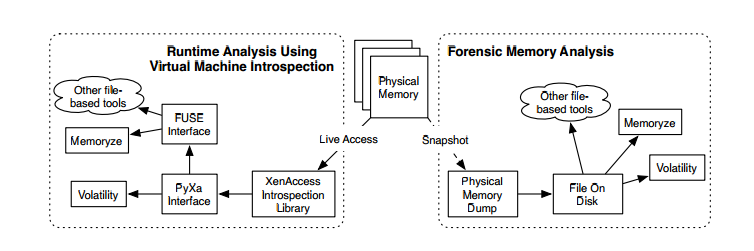
\includegraphics[width=14cm, height= 8cm ]{Figures/Figure20.png}
	\caption[Comparison of VMI and FMA]{Comparison of VMI and FMA \cite{Reference3}}
	\label{fig:Comparison of VMI and FMA}
\end{figure}

\section{INSTALLATION LIBVMI AND VOLATILITY IN KVM}
This section will introduce how to install LibVMI\&Volatility in Ubuntu14.04, where KVM virtualization platform has been 
established with success. With regard to how to establish KVM platform in Ubuntu14.04, this link 
http://adywp.blogs.unhas.ac.id/2014/05/installing-kvm-on-ubuntu-14-04/ is strongly recommended.

It is worth to mentioning that the libvirt library, installed by Ubuntu's package manager (for example by apt-get), 
does not support QMP command, which is necessary for QEMU emulator to access directly target guest's physical memory. 
Similarly, QEMU utility installed by default does not provide functions to access virtual machine's memory. Hence, 
to use LibVMI in KVM platform, the first step is to get respectively source codes for libvirt and QEMU, modify QEMU to add 
VM physical memory access code and install these utilities from source code.

To get libvirt source code, open a terminal and change into your destination directory (in our case, we plan to arrange 
all source codes required under a directory called "libvmi") and issue this command in a terminal:
\shellcmd{
		mkdir ~/libvmi \\
\#		cd ~/libvmi \\
\#		wget http://libvirt.org/sources/libvirt-1.2.6.tar.gz \\
\#		tar zxvf libvirt-1.2.6.tar.gz \\
\#		cd libvirt-1.2.6
}
When compiling and installing libvirt from source code, notice that an older version (version 1.2.2) has been already 
installed under path /usr/bin, to avoid any possible confusion, we need to update libvirt by overriding the old one:
\shellcmd{
		./autogen.sh \\
\#		./configure --prefix=/usr --localstatedir=/var --sysconfdir=/etc \\
\#		make \\
\#		sudo make install\\
\#		sudo ldconfig
}
Then, do not forget to modify libvirt configuration file and restart libvrit daemon. Modify /etc/libvirt/libvirtd.conf, uncomment this line:
\shellcmd{auth\_unix\_rw = “none”}
To restart libvirtd, type the following commands:
\shellcmd{
			sudo /etc/init.d/libvirt-bin stop \\
\#			sudo /etc/init.d/libvirt-bin start			
}
In term of QEMU, we need to firstly know why and how to modify its source code. What the patch actually does is to use 
Qemu Machine Protocol (QMP) mechanism for LibVMI to pass the GPA (Guest Physical Address), and call the internal function 
"cpu\_physical\_memory\_map" located in qemu/exec.c in Qemu, and finally get the mapped HVA (Host Virtual Address) back. 
More details about how to write a patch for a certain version of QEMU are available in this link:
\url{http://ytliu.info/blog/2014/03/27/kvm-support-in-libvmi}. Given that a QEMU patch for QEMU 1.6 is provided, we use git
to clone branch 1.6 version of QEMU:
\shellcmd{
mkdir ~/libvmi/qemu-stable-1.6 \\
\#\indent\indent\texttt{cd qemu-stable-1.6} \\
\#\indent\indent\texttt{git init} \\
\#\indent\indent\texttt{git remote add -t state-1.6 -f origin https://github.com/qemu/qemu.git} \\
\#\indent\indent\texttt{git checkout stable-1.6}
}
Supposing that the path of patch file for QEMU 1.6 is ~/libvmi/kvm-1.6-patch.patch, to patch QEMU, issue this command:
\shellcmd{
		patch -p1 < ../kvm-1.6-patch.patch \\
\#		./configure --prefix=/usr --target-list="386-softmmu x86\_64-softmmu"		
}
By default (without –target-list option), ‘configure’ will prepare many machine type emulator, and it takes long time to compile.
\shellcmd{
		make \\
\#		sudo make install
}
In addition, to assure the functioning of LibVMI, all the following additional packages are required to be installed:
\shellcmd{
sudo apt-get install zlib1g-dev libglib2.0-dev libpixman-1-dev libfdt-dev libtool libsdl1.2-dev \\
\#		sudo apt-get install libbison-dev flex libyajl-dev check autopoint python-dev libxslt1-dev xsltproc \\
\#		sudo apt-get install libdevmapper-dev libpciaccess-dev libnl-dev w3c-dtd-xhtml libjansson-dev libfuse-dev
}
Now all prerequisites works are done to install LibVMI. To get its source code, type this command:
\shellcmd{
cd ~/libvmi \\
\#		git clone git://github.com/bdpayne/libvmi.git
}
Then change into LibVMI directory
\shellcmd{
cd libvmi
\#		./autogen.sh \\
\#		./configure \\
\#		make \\
\#		sudo make install \\
\#		sudo ldconfig
}
If all required packages are present in system, after running. /configure command, we should the output shown in Figure 
\ref{fig:Output of ./configure for LibVMI}.
\begin{figure}[htbp]
	\centering
		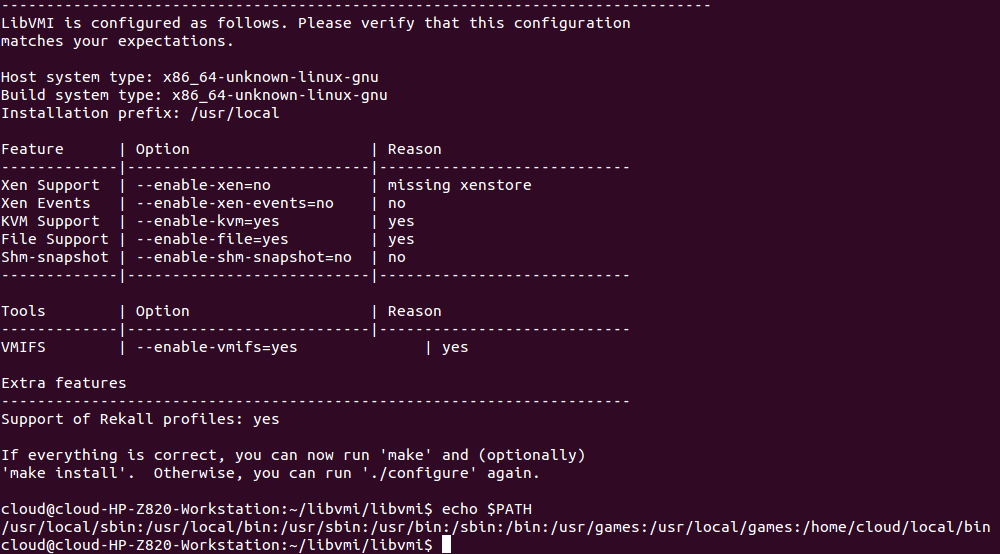
\includegraphics[width=14cm, height= 10cm ]{Figures/Figure21.png}
	\caption[Output of ./configure for LibVMI]{Output of ./configure for LibVMI}
	\label{fig:Output of ./configure for LibVMI}
\end{figure}

LibVMI will be installed in path /usr/local/bin. It is worth to mentioning that after update of QEMU and libvirt, 
some KVM's virtual machines, which are installed under the help of older libvirt version, will encounter some problems 
to start. This is caused by the name convention difference in virtual machine XML configuration file.

After modifying target guest virtual machine's configuration, reload it to take effect
\shellcmd{sudo service livirt-vin reload}
Then all guests who have problems to start now could work normally as before. To verify the correct installation of 
LibVMI, we need to execute the example "process-list" shipped with LibVMI. This example needs some configuration file 
to work. The details on this file can be read here: \url{https://code.google.com/p/vmitools/wiki/LibVMIInstallation}. In
our situation, we put this configuration "libvmi.conf" under path ~/etc/. The most difficult task to complete the LibVMI 
configuration file is how to get "offset" value for certain kernel data structure. Fortunately, LibVMI has provided 
specific tools for this task.

Ignoring the process of how to edit this file, the following is the part of libvmi.conf:

vm2 \{\\
	ostype = "Linux";\\
	sysmap = "/home/cloud/etc/System.map-2.6.32-38-generic";\\
	linux\_name = 0x30c;\\
	linux\_tasks = 0x1d8;\\
	linux\_mm = 0x1f4;\\
	linux\_pid = 0x214;\\
	linux\_pgd = 0x28;\\
\}

vm1\{
\\
	ostype = "Windows";
\\
    	win\_tasks   = 0x188;
\\
    	win\_pdbase  = 0x28;
\\
   	win\_pid     = 0x180;\\
    	win\_pname   = 0x2e0;\\
\}

Executing the following command, we should see the list of currently running processes inside vm2.
\shellcmd{sudo process-list vm2}
From now on, we could say that LibVMI has been successfully installed in our KVM virtualization platform. LibVMI allows 
cooperating with Volatility Forensic Memory Analysis framework by providing a python wrapper; due to the fact that 
Volatility is written in Python while LibVMI in C. To install this Python wrapper, change into the folder ``pyvmi'' and 
issue commands:
\shellcmd{python setup.py build \\\#		sudo python setup.py install}
\begin{figure}[htbp]
	\centering
		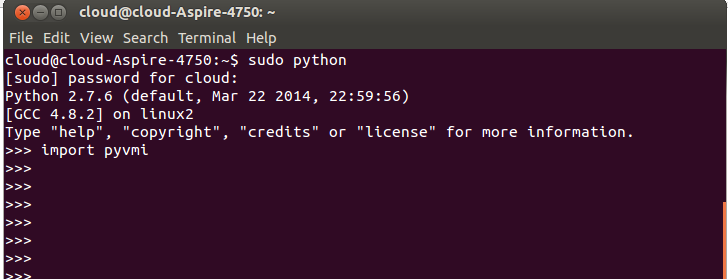
\includegraphics[width=14cm, height= 10cm ]{Figures/Figure22.png}
	\caption[Import Pyvmi in Python interactive Shell]{Import Pyvmi in Python interactive Shell}
	\label{fig:Import Pyvmi in Python interactive Shell}
\end{figure}

Run python in a terminal and try to import pyvmi module, nothing output means that LibVMI has been encapsulated as module into Python. 
Now we could invoke LibVMI API in Python script.

Now it’s time to get Volatility.
\shellcmd {cd ~/libvmi}
\shellcmd {wget https://volatility.googlecode.com/files/volatility-2.3.tar.gz}
\shellcmd{tar zxvf volatility-2.3.tar.gz}
\shellcmd{cd volatility-2.3.tar.gz}

In term of installing Volatility's code, we have two choices, each has its own advantages and disadvantages.

1) Extract the archive and run setup.py. This way is useful when we want to import Volatility as module in Python script, however, it is not 
convenient for upgrading or uninstalling.


2) Extract the archive to a directory of your choice. When you want to use Volatility just do python /path/to/directory/vol.py. This is a 
cleaner method since no files are ever moved outside of your chosen directory, which is convenient for possible update of Volatility in the 
future. The cost is that Volatility could not be used as a library in Python script.

For our case, we choose to run setup.py for the purpose of using Volatility as a module. Now we manage to install LibVMI and Volatility in 
our KVM experimentation platform. The following section will talk about my manipulation.

\section{Explore Volatility with LibVMI}
This section is used to record the exploration course of exploring the usage of Volatility and LibVMI for running KVM virtual machines. 
The first section is about a general introduction about Volatility.
\subsection{Introduction about Volatility}
The Volatility Framework is a completely open-source collection of tools, implemented in Python under the GNU General Public License, 
for the extraction of digital artifacts from volatile memory (RAM) samples. The extraction techniques are performed completely independent 
of the system being investigated but offer visibility into the runtime state of the system. The framework is intended to introduce people 
to the techniques and complexities associated with extracting digital artifacts from volatile memory samples and provide a platform for 
further work into this exciting area of research. The official documentation is very complete and is available here
: \url{http://code.google.com/p/volatility/wiki/VolatilityIntroduction?tm=6}.
\subsection{Volatility Usage}
Since the installation is introduced previously, here we talk about directly the usage of this powerful tool. Briefly, the most basic 
volatility commands are constructed as shown below:
\shellcmd{python path/to/vol.py [plugin] -f [image] --profile=[profile]}
Placeholder [plugin] in above command line represents the functionality provided by Volatility. For example “pslist” plugin allows listing all 
currently running processes. [image] means the path to the target memory dump. It could be in various types depending supported address 
space, such as raw dd style format or LiME \cite{Reference35} format for Linux. [profile] indicates which memory layout or kernel data structure will 
be used to investigate input memory sample file. One reason why Volatility is so useful and popular is due to complete and predefined 
profile for Windows.

Replace plugin with the name of the plugin to use (pslist, netscan, linxu\_netstat,etc.), image with the file path to your memory image, 
and profile with the name of the profile (such as Win7SP1x64, the default profile is always WinXPSP3x86).

For example, imaging a Windows guest memory dump named “win7.dd” is at our disposal. Now we want to investigate which network connections are established.  
The following command is used to achieve this:
\shellcmd{sudo python vol.py netscan -f /path/to/win7.dd –profile=Win7SP1x86}
For everything beyond this example, such as controlling the output format, listing the available plugins and profiles, or supplying 
plugin-specific options, see the rest of the text below. https://code.google.com/p/volatility/wiki/VolatilityUsage23


\subsection{Plugin}
As mentioned above, the functionalities of Volatility are in implemented in form of plugin and could be extended. Initially, 
Volatility is used uniquely for Windows memory analysis, thus it provides up to now variety of plugins for Windows. This plugins could 
be grouped into the those categories shown in Figure \ref{fig:Windows Core Plugin List}:

\begin{figure}[htbp]
	\centering
		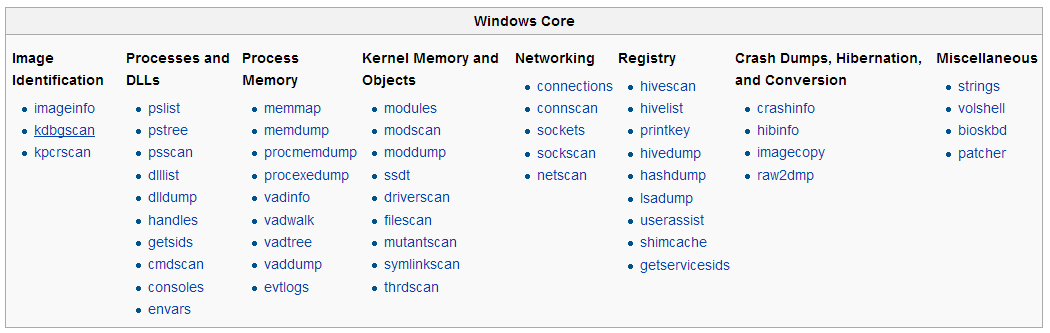
\includegraphics[width=14cm, height= 10cm ]{Figures/Figure23.png}
	\caption[Windows Core Plugin List]{Windows Core Plugin List \cite{Reference13}}
	\label{fig:Windows Core Plugin List}
\end{figure}

Thus with Volatility, we could get a rather clear visibility for the security or monitoring purpose, for the running state of the target
machine if we have its memory sample file.

\begin{figure}[htbp]
	\centering
		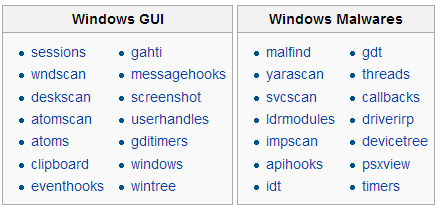
\includegraphics[width=14cm, height= 10cm ]{Figures/Figure24.png}
	\caption[Windows GUI and Malware Plugins List]{Windows GUI and Malware Plugins List \cite{Reference13}}
	\label{fig:Windows GUI and Malware Plugins List}
\end{figure}

Before Volatility version 2.1, Volatility does not support memory forensic analysis for Linux. At the moment, another FMA tool called 
Volitilinux is used for this task. Volitilinux could be regarded as counterpart of Volatility for Linux. From Volatility version 2.2, 
Volatility has incorporated Volitlinux’s functionality and has a more wide range OS support.

In term of Linux, available plugins are resumed in Figure \ref{fig:Linux Memory Forensic Plugin}.
\begin{figure}[htbp]
	\centering
		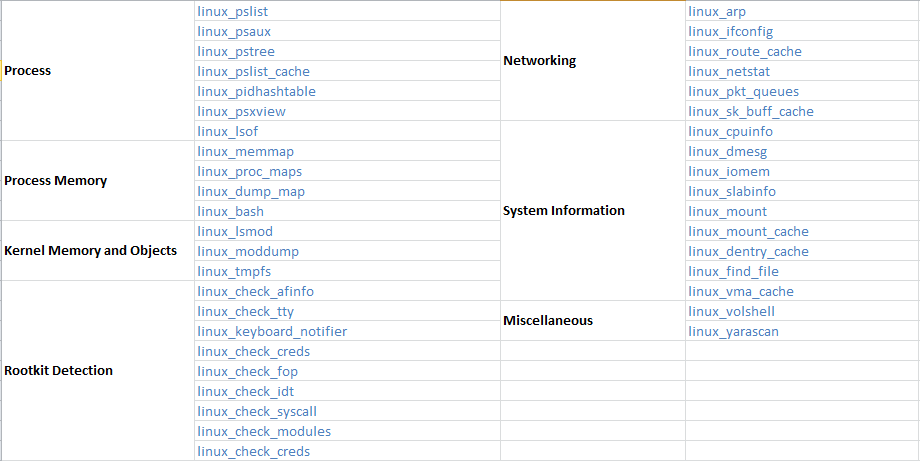
\includegraphics[width=14cm, height= 10cm ]{Figures/Figure25.png}
	\caption[Linux Memory Forensic Plugin]{Linux Memory Forensic Plugin \cite{Reference36}}
	\label{fig:Linux Memory Forensic Plugin}
\end{figure}

In this article, we will not present all the available plugins.
Here we pick up some typical and useful command to present the power of Volatility. 
For example, Figure \ref{fig:Volatility netscan(for windows) plugin's output} demonstrates that “netscan” command helps us to get all 
the currently established network connections with their corresponding process.

\begin{figure}[htbp]
	\centering
		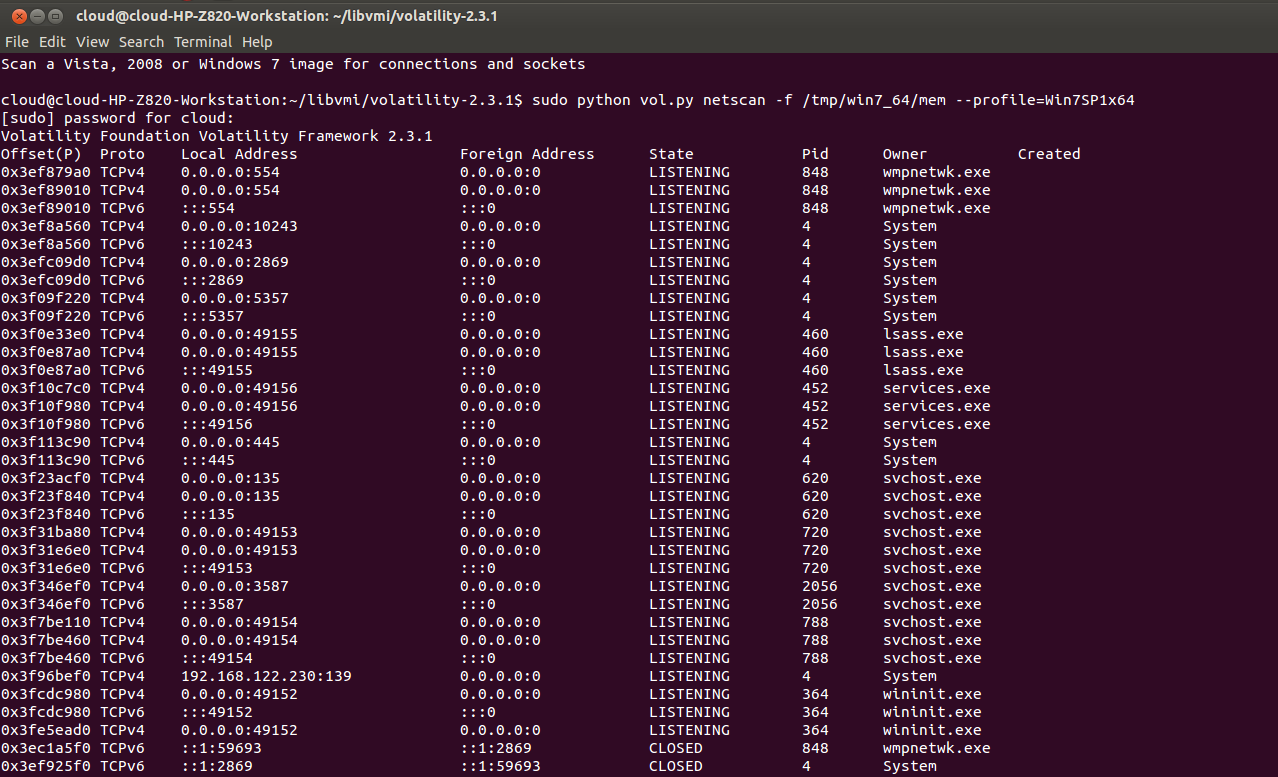
\includegraphics[width=14cm, height= 10cm ]{Figures/Figure26.png}
	\caption[Volatility netscan(for windows) plugin's output]{Volatility netscan(for windows) plugin's output}
	\label{fig:Volatility netscan(for windows) plugin's output}
\end{figure}

Up to now, the actual list of available plugins is long and grows quickly due to the strong development community. 
We could leverage these plugins to develop our own VMI applications or extend the list of available plugins.

\subsection{Profile}
Volatility is actually an out-of-band method to mitigate the semantic gap, due to the fact that before executing forensic memory, 
some configuration files about operating system kernel data structures are required. 
This kind of configuration file is usually called “Profile”. 
The command “sudo python path/to/vol.py --info | grep -i Profile” returns the profile list 
(Figure \ref{fig:Supported Profile List in Our KVM Platform})currently supported by Volatility.

\begin{figure}[htbp]
	\centering
		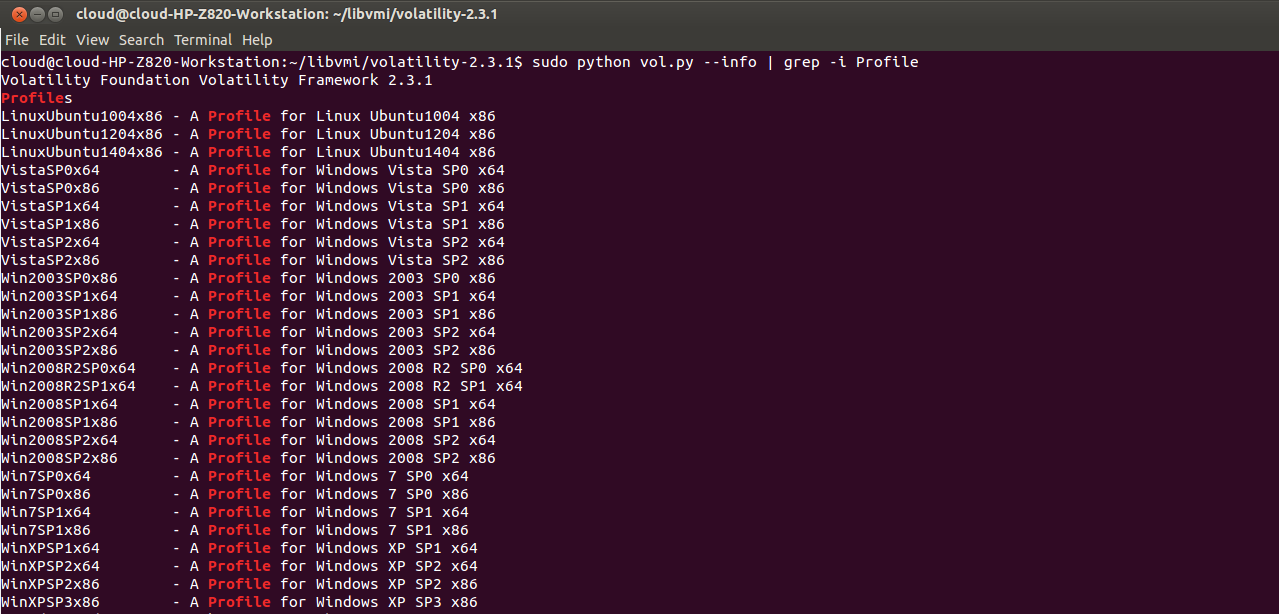
\includegraphics[width=14cm, height= 10cm ]{Figures/Figure27.png}
	\caption[Supported Profile List in Our KVM Platform]{Supported Profile List in Our KVM Platform}
	\label{fig:Supported Profile List in Our KVM Platform}
\end{figure}

Those who need an attention is, Volatility by default has provided profiles for all existing Windows series OS, 
because Windows OS’s kernel versions are relatively stable. For Windows guest memory analysis, no additional steps are necessary to 
generate the corresponding profile. This is not the case for Linux. Since there exists all kinds of Linux distribution and Linux’s 
kernel is always in constant evolution, we need to create a unique profile for every kernel version (2.6.x, 3.x, etc.), every 
distribution (such as Ubuntu/Fedora/CentOS,etc.). Plenty of online tutorials are available for this subject, for example: 
\url{https://code.google.com/p/volatility/wiki/LinuxMemoryForensics}.

\subsection{Address Space}
The address space notion is used to describe different memory dump. 
For different memory dump format, corresponding address space should be used to assure the correct functioning of memory analysis. 
It’s not necessary to indicate which address space is used when calling a certain Volatility command. 
Volatility applies a heuristic algorithm to automatically choose the appropriate address space for input memory dump. 
The following figure has shown all support address space in our KVM virtualization platform.

\begin{figure}[htbp]
	\centering
		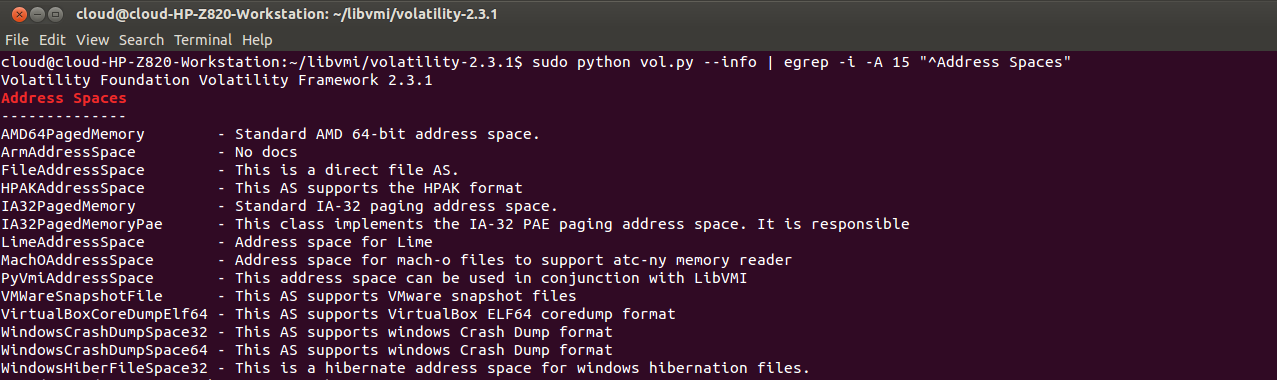
\includegraphics[width=14cm, height= 7cm ]{Figures/Figure28.png}
	\caption[Volatility Supported Address Space]{Volatility Supported Address Space}
	\label{fig:Volatility Supported Address Space}
\end{figure}

The address space could be also extended by developing special plugin for special memory dump. 
For example, to make Volatility to support LibVMI’s API, the author of LibVMi has developed a special address space plugin called 
“PyVmiAddressSpace”. It’s only necessary to copy Python script “pyvmiaddressspace.py” into the following directory under 
Volatility 2.3: volatility/plugins/addrspaces/.

\section{Cooperation with LibVMI}
Volatility is designed to work on forensic memory snapshots. In this mode, a forensic analyst would take a physical memory image from
a target machine, and then use Volatility to extract useful information from that image. However, since Volatility already contains 
significant information on the Windows/Linux memory layout and because Volatility greatly simplifies the development of memory analysis 
tools, LibVMI development team tried to integrate Volatility with LibVMI to facilitate analysis on a running virtual machine \cite{Reference8}. Thanks
to their great job, now a “VMI application-LibVMI-Volatility” tool chain has been established to simplify the development of VMI application.
In this section, we talk about how they make Volatility work directly on a live virtual machine.

In fact, LibVMI is implemented in C and we should develop some VMI applications (out-of-band) with its C library. With the popularity of 
Python in VMI research domain, LibVMI also provides a Python wrapper called PyVMI to allow LibVMI being used by Python script, such as 
Volatility framework. Their effort has formed the software stack shown in Figure \ref{fig:Software stack with PyVMI wrapper on top of the C language LibVMI library}.

\begin{figure}[htbp]
	\centering
		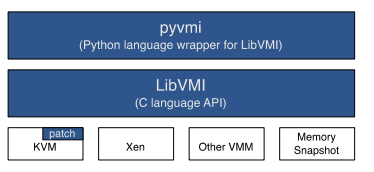
\includegraphics[width=14cm, height= 7cm ]{Figures/Figure29.png}
	\caption[Software stack with PyVMI wrapper on top of the C language LibVMI library]
	{Software stack with PyVMI wrapper on top of the C language LibVMI library \cite{Reference6}}
	\label{fig:Software stack with PyVMI wrapper on top of the C language LibVMI library}
\end{figure}

With Pyvmi, LibVMI could be used a module in Python script. Now, we should consider how to allow Volatility functioning on a live virtual machine. 
To do this, LibVMI provides two mechanisms.

\subsection{PyVMI Address Space Plugin}
This first mechanism is using a special address space plugin called “PyVMIAddressSpace”. Figure \ref{fig:Software stack with Volatility address space plugin}
shows how Volatility plugins could leverage this address space plugin to cooperate with LibVMI. Supposing we want to investigate which 
processes are currently running in target guest named “win7\_32bit”, this command could help us:
\shellcmd{sudo python path/to/vol.py pslist -l vmi:///win7\_32bit --profile=Win7SP1x86}
Although LibVMI development team announced that with PyVMI address space plugin, all Volatility plugins will work on a running virtual 
machine. With my manipulation we encountered some unexpected problems. Firstly, this plugin works for almost all Windows plugin while 
plants for some Linux plugins such as linux\_netstat. Secondly, sometimes (not always) after applying for example netscan plugin for a 
Windows, I found that the volume of log file (under path /var/log/libvirt/qemu) possibly augmented until all root file system’s disk 
space was all consumed. To solve this problem, I have posed this problem in LibVMI google discussion group but not received any response. 
I don’t know this problem is specific to my KVM platform. Therefore, at least in my work environment, PyVMI address space plugin is not 
recommended compared to its alternative.

\begin{figure}[htbp]
	\centering
		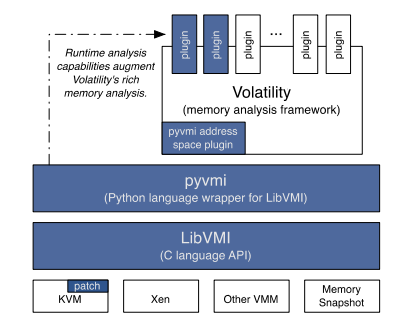
\includegraphics[width=14cm, height= 9cm ]{Figures/Figure30.png}
	\caption[Software stack with Volatility address space plugin]{Software stack with Volatility address space plugin \cite{Reference6}}
	\label{fig:Software stack with Volatility address space plugin}
\end{figure}

\subsection{Pyvmifs.py script}
The second mechanism is firstly mounting virtual machine’s physical memory as a regular file then using Volatility to analyze this 
memory file as if it were static. LibVMI has provided a special Python script to achieve this task. Its usage is:
\shellcmd{sudo python path/to/pyvmifs.py -o allow\_other -o domain=GUEST\_NAME path/to/mount/point}
Still take our Windows guest “win7\_32bit” as example. After above invocation, its physical memory is mounted under path 
/tmp/win7\_32bit/mem. Then invoke for example pslist plugin to get the running process list:
\shellcmd{sudo python path/to/vol/py pslist -f /tmp/win7\_32bit/mem --profile=Win7SP1x86}
Different with pyvmi address space plugin, the simple Python script works well and poses none problem.

\section{Experimentation Result}
To simplify the usage of Volatily, we have created a seperated Python script "demo.py" in /home/cloud/libvmi/script. For its usage,
we could issue command under the directory in question:
\shellcmd{sudo python demo.py -h}
With LibVMI+pyvmifs.py+volatility, we could run all interesting plugins for our KVM Windows/Linux virtual machines. 
Figure shows the resume of execution of under Windows 7 x86/64 and Ubuntu 10.04 x86.

\begin{figure}[htbp]
	\centering
		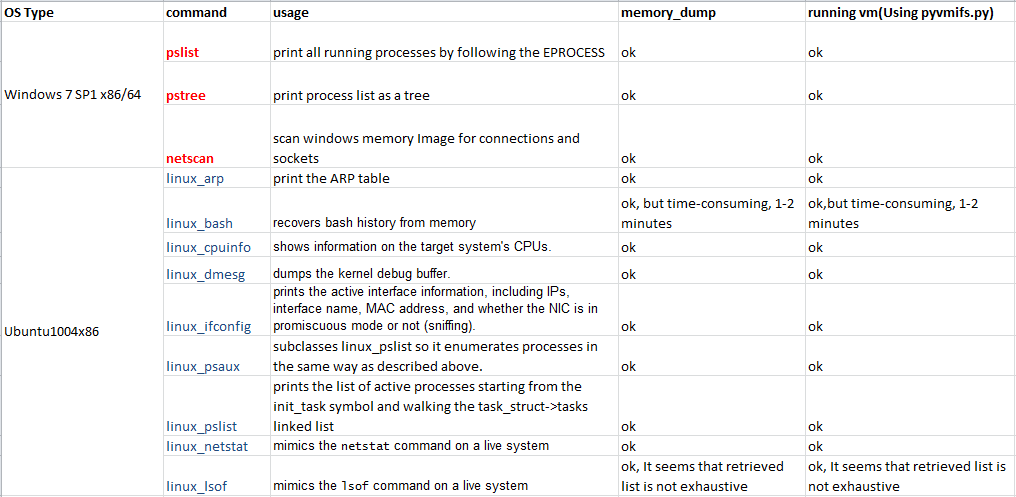
\includegraphics[width=14cm, height= 9cm ]{Figures/Figure31.png}
	\caption[Experimentation Result of Volatility Plugins in KVM Platform]{Experimentation Result of Volatility Plugins in KVM Platform}
	\label{fig:Experimentation Result of Volatility Plugins in KVM Platform}
\end{figure}

7.7Limit of Volatility\&LibVMI

Although Volatility presents various advantages in memory forensic analysis domain, its disadvantages are still obvious in the context 
of Virtual Machine Introspection: Volatility is applied uniquely to memory analysis, whereas Virtual Machine Introspection could also 
cover introspection on virtual CPU or virtual disk. Fortunately, LibVMI and libguestfs \cite{Reference38} could come to cover this shortage. 
LibVMI allows monitoring the running state of vCPU and libguestfs library is able to access and modify virtual machine’s disk image. 








% Chapter Template

\chapter{VIRTUOSO INSTALLATION AND MANIPULATION} % Main chapter title

\label{Chapter8} % Change X to a consecutive number; for referencing this chapter elsewhere, use \ref{ChapterX}

\lhead{Chapter 8. \emph{VIRTUOSO INSTALLATION AND MANIPULATION}} % Change X to a consecutive number; this is for the header on each page - perhaps a shortened title

Although forensic memory analysis community has developed plenty of utilities which could be leveraged for VM introspection, 
VMI applications based on these utilities such as volatility plugin, are still not able to be applied conveniently in for example 
operator provided cloud environment. The reason is obvious: the approach strongly depends on the stability of target VM kernel and need much
more humain effort. Once update or patch is applied to monitored guest’s kernel, these VMI applications may need to be adapted. To remedy this 
mentioned problem, we need to think out of box. An interesting and fundamental insight is: it is typically trivival to write programs inside 
the guest OS that compute the desired information by querying the built-in APSs. Logcially and naturally, people think to how to reutulize 
the existing API(binary code) in the guest to automate the generation of VMI tools. Not only the binary code, the execution contex under some
circumstance also could be leveraged to do VMI, we call this philosophy as "Reutilization Pattern". 

Nowdays there exist some famous and attractive research efforts based on reutilizatin pattern, such as VIRTUOSO\cite{Reference27}, 
EXTERIOR\cite{Reference29}, HyperShell\cite{Reference31},etc.. Among all these VMI techonologies, HyperShell is the most attractive: it provides
a hypervisor layer guest OS shell that has all of the functionalities of a traditional shell, but offers better automation, uniformity and 
centralized management. However, its source code is not accessible, but I still recommand to give it some attention.
Because VIRTUOSO is the unique open source tool in this domain, therefore, we still have to  explore VIRTUOSO to hava a more depper
knowledge about reutilization pattern.

\section{Implementation of VIRTUOSO}
To illustrate our disscusion about VIRTUOSO(installation, execution and assesse), it is better to have a general introduction about
its design and implementation. As we talked before, VIRTUOSO's objective is how to translate a guest-OS program into a form that could run
outside of its native environment. To achevie this, VIRTUOSO relies on dynamic analysis to capture all the codes executed while the target
program is runing. Meanwhile, VIRTUOSO leverages dynamic slicing technique to identify the exact set of instructions required to compute the
introspection. In addition, due to the dynamic analysis nature of VIRTUOSO, it is supposed to have a trace merging algorithm to merge the
gathered traces from multiple time execution. In one word, VIRUOSO's innovation lies in three key techniques : dynamic analysis, dynamic 
slicing and trace emerging.

Generally speaking, VIRTUOSO creates introspection tools for an operating system by converting in-guest programs, which query guest OS's
public APIs, into hypervisor-level programs that reproduce the almost same result with in-guest utilises. This process could be finished
in three phases: training phase, analysis phase and runtime phase.

As shown in Figure \ref{fig:VIRTUOSO's Component and Architecture}, training phase is conducted by "Trace Logger" component in a trusted VM , 
which has the same OS and kernel version with clients' OS. Trace logger is acutally an modified version of QEMU 0.9.1 in which logging all instructions functionality
is added. the training programs running in trusted guest are in charge of to signal the Trace Logger and inform the latter of the beginning
and end of the introspection operation. Thus, we could infer that writing a correct training program is not trivival.

The gathered traces in training phase contain the instructions of the whole system, namely, in addtion to computing the introspection quantity
, the traces also include unrelated events such as interrupt handling. we nened to excise those extraneous parts of the traces. This is the
objective of component "Trace Analyser". This anaylsis depends on dynamic data slice techinique applied on each trace. Finally, we merge the slice
results accross basic blocks and traces, producing a unified program that could be translated into an out-of-guest intro routine. In pracice, this
component is written in Python. 

The translated code could not be executed directly, il must be called with an appropriate runtime environment in which to execute. Currently, the
generated intropsection utilities are in form of Volatility plugin. Therefore, the runtime environment in current implementation of VIRTUOSO is 
Volatility.
  
\begin{figure}[htbp]
	\centering
		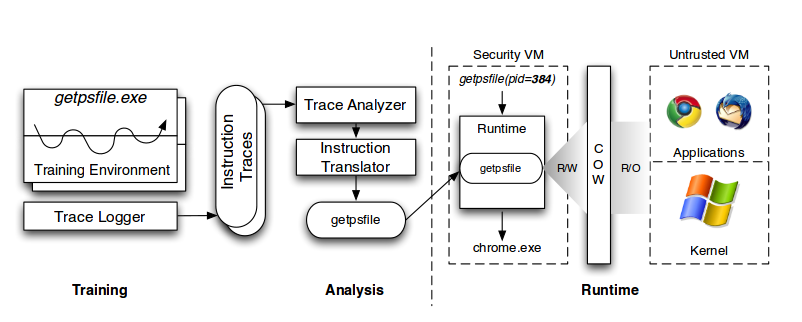
\includegraphics[width=14cm, height= 7cm ]{Figures/FigureVirtuoso.png}
	\caption{VIRTUOSO's Component and Architecture \cite{Reference27}}
	\label{fig:VIRTUOSO's Component and Architecture}
\end{figure}

\section{Installation of VIRTUOSO}

A rather detailed and helpful how-to wiki about installation of VIRTUOSO is available in the link 
\url{https://code.google.com/p/virtuoso/wiki/Installation}. Since that this wiki has not seen any update since 2012, 
we were still stuck by some unexpected problems.  As a meaningful complement to the initial how-to wiki, this tutorial aims to record 
all crossed problems and its solution in the road of VIRTUOSO exploration.

To install VIRTUOSO, 64-bit Linux system (Debian/Ubuntu preferred) and Python 2.6 or later are required. Its source code is available at 
\url{http://code.google.com/p/virtuoso/downloads/list}. After obtaining the VIRTUOSO source code, it consists of two steps to install VIRTUOSO:
install all dependencies for VIRTUOSO (gcc 3.4, QEMU 0.9.1, libdasm), compile and install iFerret.

%-----------------------------------
%	SUBSECTION 1
%-----------------------------------
\subsection{Problem 1: No SDL support for installation of QEMU 0.9.1}
The first obstacle encountered appears during the installation of QEMU 0.9.1, which is shown in Figure \ref{fig:No SDL support for installation of QEMU 0.9.1}.

\begin{figure}[htbp]
	\centering
		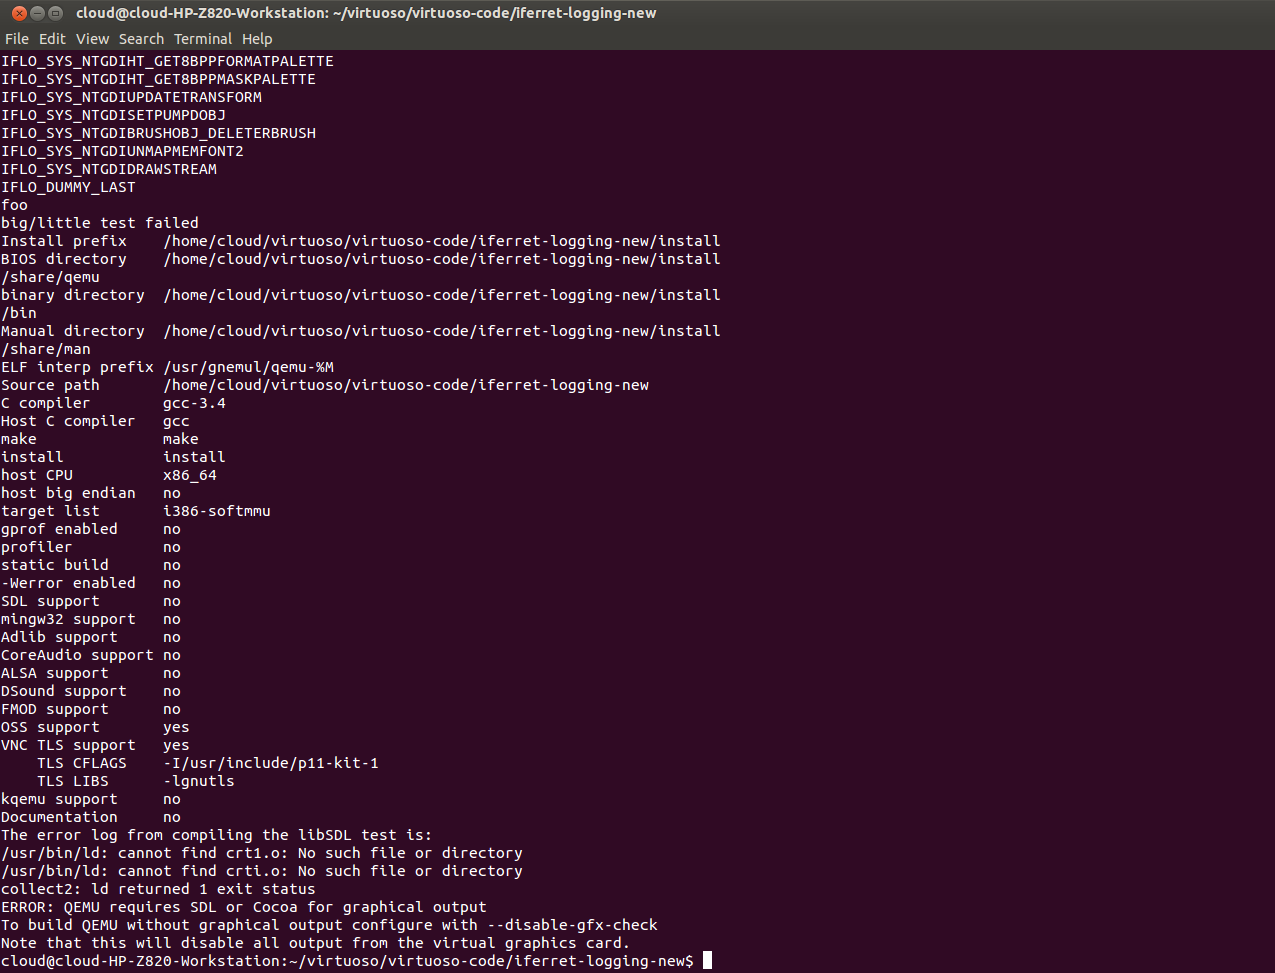
\includegraphics[width=14cm, height= 9cm ]{Figures/Figure32.png}
	\caption[No SDL support for installation of QEMU 0.9.1]{No SDL support for installation of QEMU 0.9.1}
	\label{fig:No SDL support for installation of QEMU 0.9.1}
\end{figure}

The cause of this error lies in that system could not find graphical output support for QEMU 0.9.1(notice that SDL support check's 
result is no.). After some searching online, I found a solution to this problem: It should issue the following command in the terminal a prior to
installing iFerret component of VIRTUSO:
\shellcmd{export LIBRARY\_PATH=/usr/lib/x86\_64-linux-gnu}
With this export command, system is able to find the path to libSDL library required by QEMU 0.9.1.

%-----------------------------------
%	SUBSECTION 2
%-----------------------------------

\subsection{Problem 2: iFerret compile error}
The error is occurred when we change into the 'iferret-logging-new' directory and issue 'make install' command, as shown in Figure 
\ref{fig:iFerret compile error}.

\begin{figure}[htbp]
	\centering
		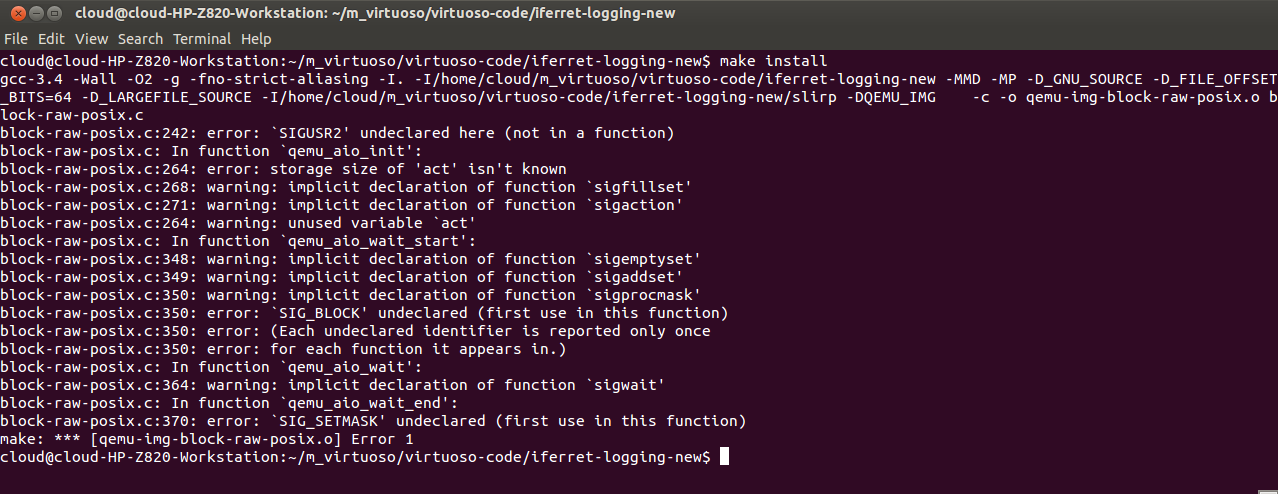
\includegraphics[width=14cm, height= 9cm ]{Figures/Figure33.png}
	\caption[iFerret compile error]{iFerret compile error}
	\label{fig:iFerret compile error}
\end{figure}

Obviously, from above figure, we could infer that there exist some bugs in source file ‘block-raw-posix.c’. After some investigation, 
this is caused by a macro definition syntax. Look at the block of code shown in Figure \ref{fig:Bloc of code causing compile error} which
causes the above error:

\begin{figure}[htbp]
	\centering
		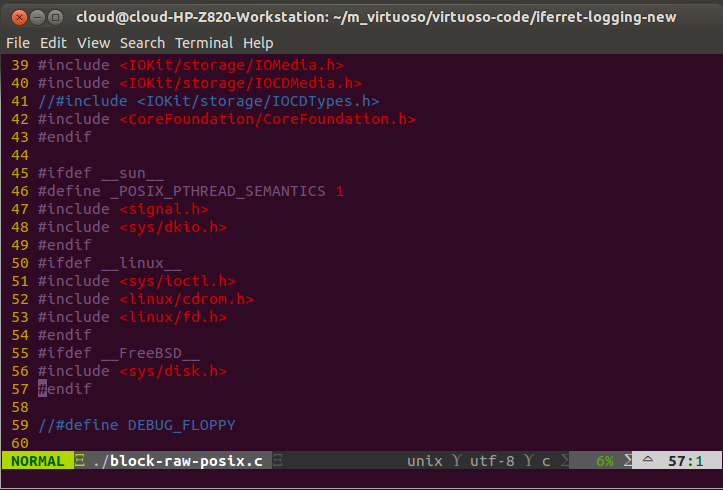
\includegraphics[width=14cm, height= 9cm ]{Figures/Figure34.png}
	\caption[Bloc of code causing compile error]{Bloc of code causing compile error}
	\label{fig:Bloc of code causing compile error}
\end{figure}

C header file ‘signal.h’ is included under some conditions. To solve this problem, it simply needs to  add one line instruction at the 
beginning of this file: \#include <signal.h>. Repeat 'make install' command, normally, no errors will appear and the installation process 
should be finished with success. Now you could give a try to VIRTUOSO following another wiki in its official site.

\subsection{Problem 3: The abort of execution of example VM image}
We follow this link \url{https://code.google.com/p/virtuoso/wiki/Walkthrough} to have a try with VIRTUOSO. Issuing the command line:
\shellcmd{install/bin/qemu -m 256 -hda haiku-r1alpha2-anyboot.qcow2 -usbdevice tablet\\ -loadvm introprog -monitor stdio -k en-us -iferret\_log 
walkthrough}
However, new error has occurred:

\begin{figure}[htbp]
	\centering
		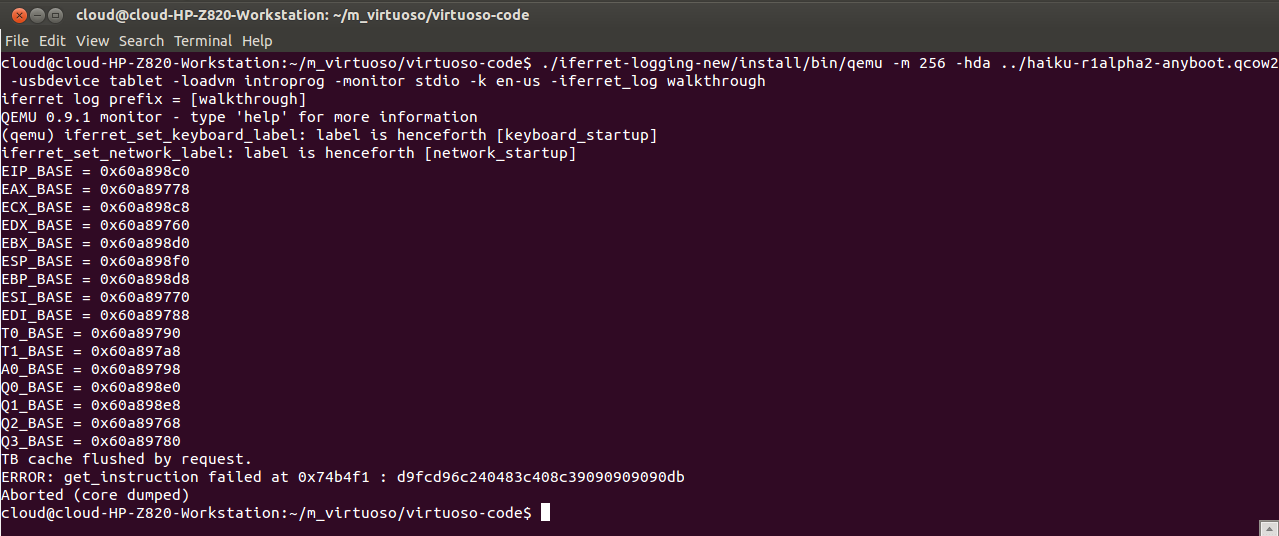
\includegraphics[width=14cm, height= 9cm ]{Figures/Figure35.png}
	\caption[Abort of execution of example VM image]{Abort of execution of example VM image}
	\label{fig:Abort of execution of example VM image}
\end{figure}

This error is not evident as others obstacles we encountered before and nothing could be found online. After one week’s effort, 
I finally got some clues about this problem to read another wiki 'limitation' at \url{https://code.google.com/p/virtuoso/wiki/Limitations},
This is caused by the fact that:

\textcolor{blue}{
  "Virtuoso makes use of libdasm to disassemble instructions (see iferret-logging-new/target-i386/translate.c for details). 
  Libdasm is missing support for some instructions, and this will cause tracing to stop and QEMU to shut down. The disassembly Virtuoso does 
  is mainly for debugging, and so these lines can be commented out if they cause trouble. I would like to switch to a more reliable disassembler 
  in the future, however."
}

Therefore, the answer to the problem is: libdasm encountered some unknown instructions in Ubuntu14.04 and forces VIRTUOSO to abort. 
To solve this, we need to identify and comment related block of code in file 'translate.c' and recompile all. Concretely, comment line 
from 3281 to 3335 in file ‘iferret-logging-new/target-i386/translator.c’ and recompile install all. 

Until now, we could take a ride with VIRTUOSO. Change into directory ‘iferret-logging-new’ and issue the following command line into a 
terminal:
\shellcmd{install/bin/qemu -m 256 -hda haiku-r1alpha2-anyboot.qcow2 -usbdevice tablet\\ -loadvm introprog -monitor stdio -k en-us -iferret\_log walkthrough}
Some explanation about above command: To prove that VIRTUOSO is OS-angostic VMI technology, we use a Haiku OS-based virtual machine image provided
by author. This virtual machine comes with a snapshot named "introprog" that has a few training programs already loaded and compiled. 
For example, we could run a training program named "enumprocs" to get the PID list of currently running process in guest virtual machine.
The execution result is shown in Figure \ref{fig:Run Training program in trusted VM}.
\begin{figure}[htbp]
	\centering
		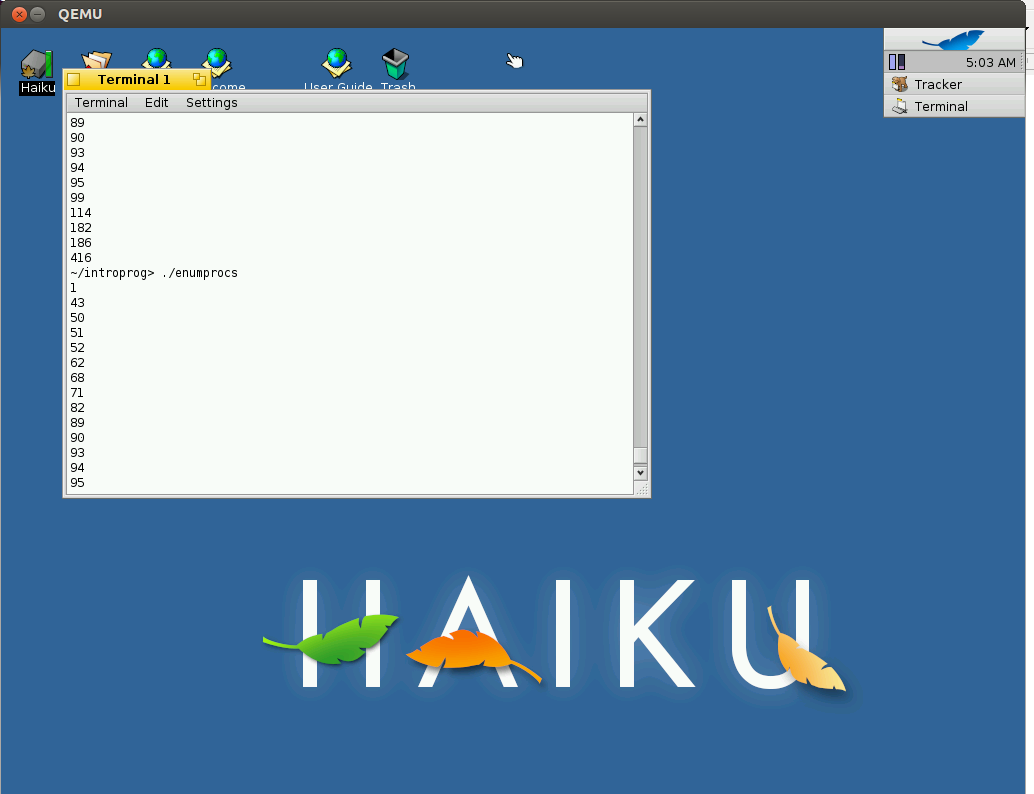
\includegraphics[width=14cm, height= 9cm ]{Figures/Figure36.png}
	\caption[Run Training program in trusted VM]{Run Training program in trusted VM}
	\label{fig:Run Training program in trusted VM}
\end{figure}

Notice that, after several times of invocation of small programs such as 'enumprocs', we observe that some execution traces files are 
generated.  Generated output file will be placed in directory where VIRTUOSO is called. (In this case, it is directory 'iferret-logging-new')

\subsection{Problem 4: IPython runtime exception when generating inspection code with VIRTUOSO}
Given that, component ‘iFerret’ of VIRTUOSO has obtained execution traces of training program, it is time to analysis trace file and 
produces the Volatility plugin. To achieve this, go to the dynslicer directory and run:
\shellcmd{./newslicer.py -o haiku ../iferrret-logging-new/walkthrough.0-17864}
Unfortunately, there comes a new error:

\begin{figure}[htbp]
	\centering
		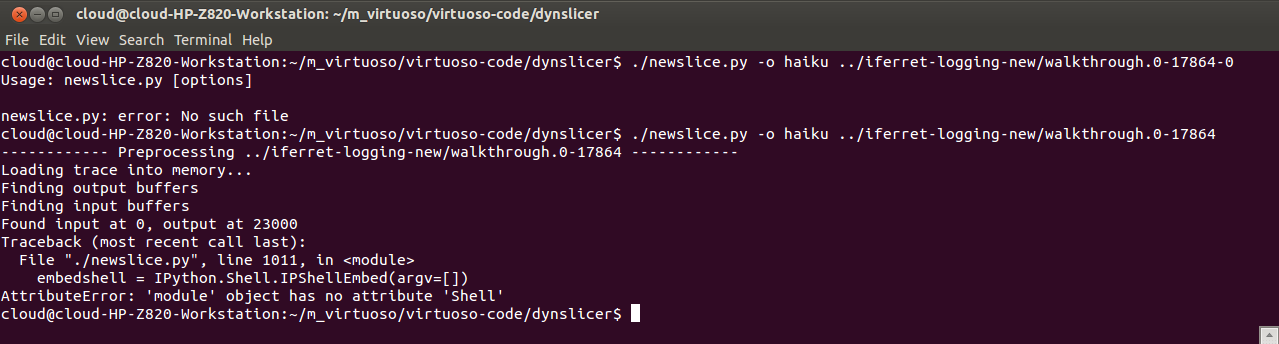
\includegraphics[width=14cm, height= 9cm ]{Figures/Figure37.png}
	\caption[IPython run exception]{IPython run exception}
	\label{fig:IPython run exception}
\end{figure}

Definitely, this is related to the IPython version installed in our workstation. A possible solution to this problem is:
\shellcmd{sudo pip uninstall ipython\\\# sudo pip --proxy=http://proxy.rd.francetelecom.fr:8080 install ipython==0.10}
Then re-execute above invocation, and output is shown in Figure \ref{fig:VIRTUOSO introspection tool generation}.
\begin{figure}[htbp]
	\centering
		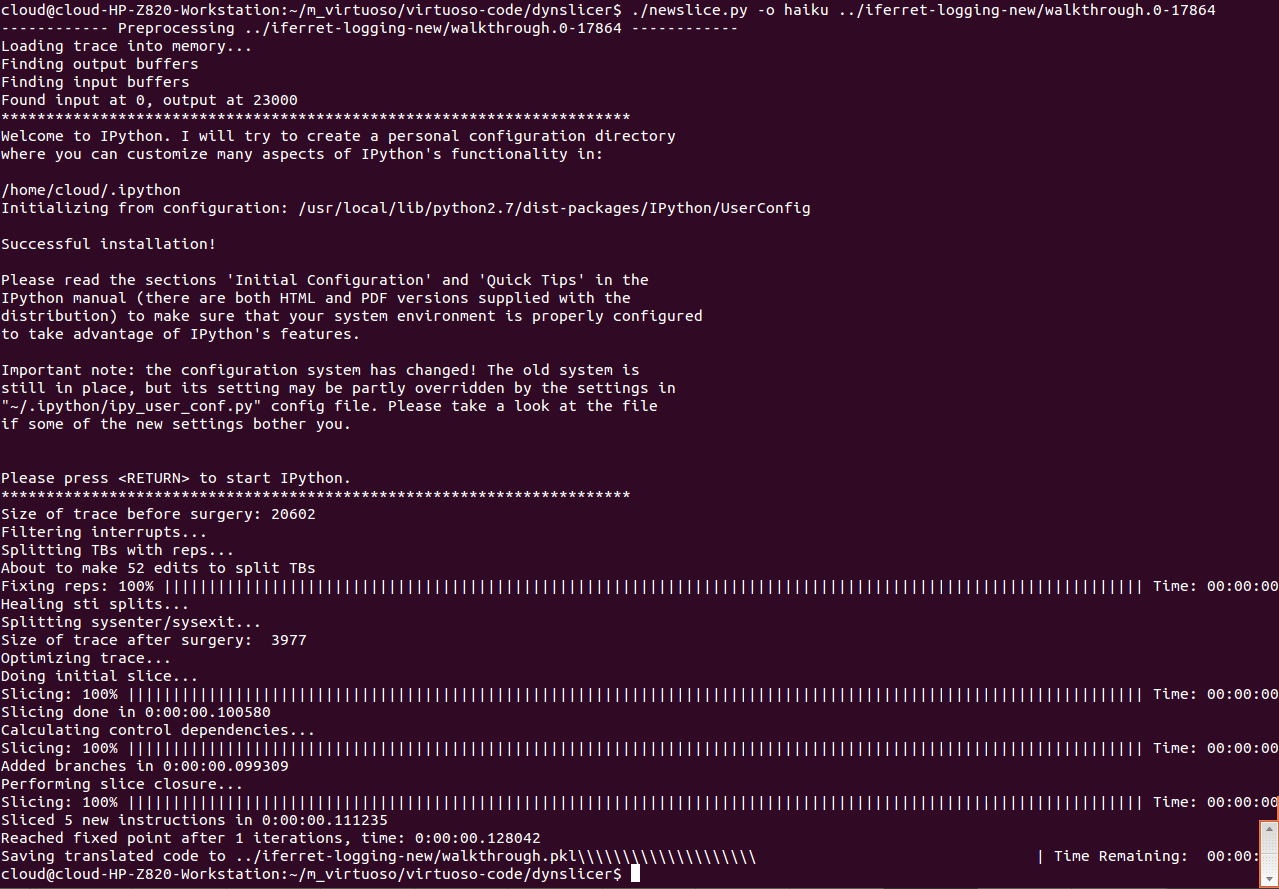
\includegraphics[width=14cm, height= 9cm ]{Figures/Figure38.png}
	\caption[VIRTUOSO introspection tool generation]{VIRTUOSO introspection tool generation}
	\label{fig:VIRTUOSO introspection tool generation}
\end{figure}
When Volatility plugin is well generated, we could profit to realize introspection job at the level of hypervisor and get mostly the 
same view as inside the monitored VM. To do this, change into volatility-1.3-Beta directory and tape the following command:
\shellcmd{./volatility newmicrodo -f ../iferret-logging-new/walkthrough.0.mem \textbackslash\\ -e ../iferret-logging-new/walkthrough.0.env\textbackslash\\ -m ../iferret-logging-new/walkthrough.pkl\textbackslash\\ -n ' [ mem.alloc(1024) ] ' -i 'def f(x): print unpack("<\%dI" \% (len(x)/4),x)'}

\begin{figure}[htbp]
	\centering
		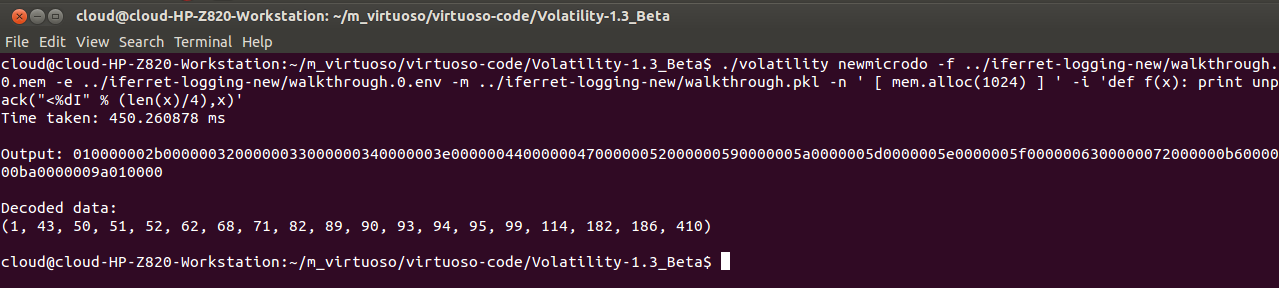
\includegraphics[width=14cm, height= 7cm ]{Figures/Figure39.png}
	\caption[VIRTUOSO introspection tool execution result]{VIRTUOSO introspection tool execution result}
	\label{fig:VIRTUOSO introspection tool execution result}
\end{figure}

\section{Assessment of VIRTUOSO}
Traditionally, the principal philosophy was to imitate the existing inspecting utility (ps, netstat command in Linux for example.) 
and rewrite the code from scratch with an intimate knowledge of OS kernel. This approach is rather intuitive but at the same time 
presents some obvious disadvantages:

\begin{itemize}
    \item Prone to import new security when writing new introspection utilities
    \item Has to adapt each time target OS kernel has some updates
    \item Need much human effort
 \end{itemize}
The greatest significance of VIRTUOSO lies in that it breaks away from conventions and leverages the reutilization of
binary code. Exception the training stage, VIRTUOSO is capable of automatically generating introspection tool with 
obtained execution traces without target OS kernel knowledge.

However, the limitation of VIRTUOSO is also evident: first, it is not still completely automatic in generating introspection
tool. VIRTUOSO still needs an expert to write the training programs to get system API execution traces in which we are
interested. This expert is supposed to have an intimate knowledge about target system API, for example, which API is used 
to get the list of running processes in Haiku operating system. When writing training program, he should also assure that
there is no process switch (context switch) during training program execution. In one word, it is a little difficult to 
write training program. Second, the range of introspection tools generated by VIRTUOSO depends on the target OS API, 
due to the fact that VIRTUOSO just simply reutilizes binary code s associated with system API. Third, VIRTUOSO is not
able to extract device I/O code or instruction, VIRTUOSO is therefore not capable of generating network-side introspection
tools. All above constraints hinder the application of VIRTUOSO in industry, but its philosophy inspired other interesting 
introspection tool, such as VMST.






%----------------------------------------------------------------------------------------
%	THESIS CONTENT - APPENDICES
%----------------------------------------------------------------------------------------

\addtocontents{toc}{\vspace{2em}} % Add a gap in the Contents, for aesthetics

\appendix % Cue to tell LaTeX that the following 'chapters' are Appendices

% Include the appendices of the thesis as separate files from the Appendices folder
% Uncomment the lines as you write the Appendices

% Appendix A

\chapter{CR3 Register Introduction} % Main appendix title

\label{AppendixA} % For referencing this appendix elsewhere, use \ref{AppendixA}

\lhead{Appendix A. \emph{CR3 Register Introduction}} % This is for the header on each page - perhaps a shortened title

The CR3 register is a typical hardware anchor [3] where we could derive some OS-level information in the context of derivative 
pattern VMI. Since our study is about how to leverage derivative pattern in monitoring network traffic on per-process basis, it’s 
better to resume the CR3’s functionality and explore its potentiality for future usage. This is the motivation of this work and the 
remainder of this article is organized as follow. In the first part, some background conceptions about memory addressing, involved 
in the functioning of CR3 register, will be presented. Subsequently, we talk about how CR3’s functionality specified in Intel 
developer manual [2] and helps in translating a linear address into a physical address. In the end, we address how CR3 register 
is leveraged to derive or infer system process information and its potentiality in network traffic monitoring. 

\section{Background \cite{BookLinuxKernel}}
To well understand the functionality of CR3 register, some basic and related conceptions about memory addressing should be kept in
mind.

\begin{itemize}
 \item\textbf{Logical Address}: consists of a segment and an offset, included in the machine language instructions to specify the address of an 
operand or an instruction.
 \item\textbf{Linear Address}: also known as virtual address, a single 32 bits unsigned integer that can be used to address up to 4GB. Their values
range from 0x00000000 to 0xffffffff.
 \item\textbf{Physical Address}: used to address memory cell in memory chips.
 \item\textbf{MMU}: Memory Management Unit, a hardware circuit integrated in x86 architecture and it consist of two parts:  
Segmentation Unit helping CPU translate a logical address into a linear address and Paging Unit capable of transforming a linear
address into a physical address.
\end{itemize}

\begin{figure}[htbp]
	\centering
		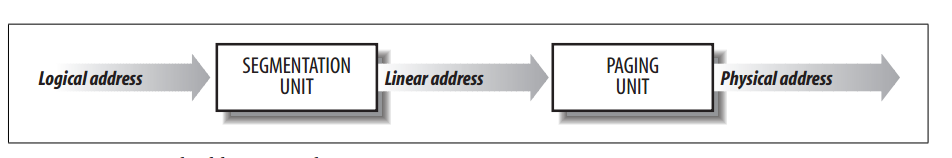
\includegraphics[width=13cm, height= 4cm ]{Figures/FigureAppendix1.png}
	\caption{Logical Address Translation \cite{BookLinuxKernel}}
	\label{fig:Logical Address Translation}
\end{figure}

Segmentation has been included in 80x86 microprocessors to encourage programmers to split their applications into logically related
entities, such as subroutines or global and local data areas. However, Linux uses segmentation in a very limited way. In fact, 
segmentation and paging are somewhat redundant, because both can be used to separate the physical address spaces of processes: 
segmentation can assign a different linear address space to each process, while paging can map the same linear address space into 
different physical address spaces. Linux prefers paging to segmentation.

\section{Functionality of CR3 Register \cite{BookIntelManuel}}
CR3 register is a control register integrated in CPU. Along with other control registers such as CR0, CR1, CR2, CR3 and CR4, they 
are used to determine operating mode of the processor and the characteristics of the currently executing task. This section presents
control register in the perspective of processors.

\begin{figure}[htbp]
	\centering
		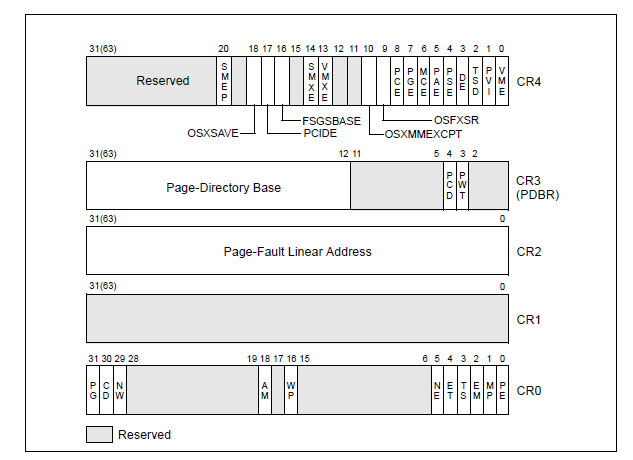
\includegraphics[width=13cm, height= 8cm ]{Figures/FigureAppendix2.png}
	\caption{Control Register Architecture \cite{BookIntelManuel}}
	\label{fig:Control Register Architecture}
\end{figure}

Figure \ref{fig:Control Register Architecture} presents the four control registers’ architecture. Their respective functionalities are
summarized below, and each architecturally defined control field in these control registers are described individually.

\begin{itemize}
 \item\textbf{CR0}: contains system control flags that control operating mode and states of the processor.
 \item\textbf{CR1}: reserved.
 \item\textbf{CR2}: contains the page-fault linear address (the linear address that caused a page fault).
 \item\textbf{CR3}: contains the physical address of the base of the paging-structure hierarchy and two flags (PCD and PWT). Only the
 most-significant bits (less the lower 12 bits) of the base address are specified; the lower 12 bits of the address are assumed to be
 0. The first paging structure must thus be aligned to a page (4-KByte) boundary. The PCD and PWT flags control caching of that paging
 structure in the processor’s internal data caches (they do not control TLB caching of page-directory information). CR3 register works
 on condition that VIRTUAL ADDRESSING feature is enabled, which means that PG bit is set in CR0.
 \item\textbf{PCD}: Page-level Cache Disable (bit 4 of CR3) — Controls the memory type used to access the first paging structure of 
 the current paging-structure hierarchy. This bit is not used if paging is disabled, with PAE paging, or with IA-32e paging if CR4.
 PCIDE=1. Please refer to Section 4.9: “Paging and Memory Typing” in reference [] to get more information.
 \item\textbf{PWT}: Page-level Write-Through (bit 3 of CR3) — Controls the memory type used to access 
\end{itemize}

\section{Functioning of CR3 Register in Memory Addressing}
Figure \ref{fig:Paging by 80x86 Processors} well explains how MMU uses CR3 register to translate a linear address into a physical one.
The 32 bits linear address can be divided into 3 parts: Directory (the most significant 10 bits), Table (the intermediate 10 bits) and
Offset (the least significant 12 bits). The physical address of the Page Directory in use is stored in a control register named CR3. 
The Directory field within the linear address determines the entry in the Page Directory that points to the proper Page Table. The 
address’s Table field, in turn, determines the entry in the Page Table that contains the physical address of the page frame containing
the page. The offset field determines the relative position within the page frame.

\begin{figure}[htbp]
	\centering
		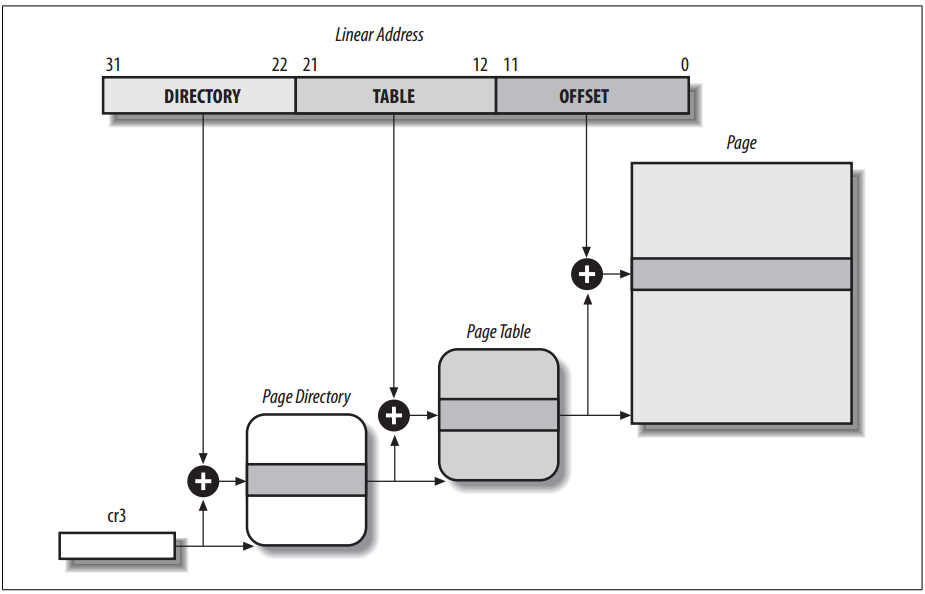
\includegraphics[width=13cm, height= 8cm ]{Figures/FigureAppendix3.png}
	\caption{Paging by 80x86 Processors}
	\label{fig:Paging by 80x86 Processors}
\end{figure}

Since the CR3 register holds the address of the top-level Page Directory for the current context and a single address space is active
per processor at any given time, the physical address stored in CR3 register could be used to represent its unique corresponding 
process. This is the theoretical base for that CR3 could be profited in the derivative pattern. For example, a new CR3 value means 
a new process has been created, a transition from one to another value in CR3 means that a context switch (process switch) has 
occurred. Antfarm \cite{Reference4} has leveraged this characteristic to enumerate all executing processes, monitor the creation, switch and exit of 
process. However, in Antfarm, cause of the limitation of derivative pattern, we could just get its page directory base address and 
executing time for each identified process. Due to the lack of semantic knowledge for kernel memory, it is impossible to get more 
detailed information (such as PID, process name, etc.) about identified processes. Based on Antfarm, Lycosid \cite{Reference9} whose 
objective is to detect the hidden malicious processes has been developed. Its idea is to compare a process list deduced by low-level 
hardware with that obtained by some system utility such as UNIX command “ps”. In case of inconsistency about process number, Lycosid
infers the presence of hidden processes in monitored VM and identify those processes in a statistical manner.














%\input{Appendices/AppendixB}
%\input{Appendices/AppendixC}

\addtocontents{toc}{\vspace{2em}} % Add a gap in the Contents, for aesthetics

\backmatter

%----------------------------------------------------------------------------------------
%	BIBLIOGRAPHY
%----------------------------------------------------------------------------------------

\label{Bibliography}

\lhead{\emph{Bibliography}} % Change the page header to say "Bibliography"

\bibliographystyle{unsrtnat} % Use the "unsrtnat" BibTeX style for formatting the Bibliography

\bibliography{Bibliography} % The references (bibliography) information are stored in the file named "Bibliography.bib"

\end{document}  